%% MDPI Article Template — Future Internet
%% Converted from IEEEtran v3 for Overleaf submission
%% Overleaf project: https://www.overleaf.com/6211227512rwjwdnjytkcm#4c379d

\documentclass[futureinternet,article,submit,pdftex,moreauthors]{Definitions/mdpi}

%=================================================================
% Packages (supplementary — MDPI class loads most essentials)
\usepackage{amsmath,amssymb,amsfonts}
\usepackage{graphicx}
\usepackage{booktabs}
\usepackage{float}
\usepackage{tikz}
\usepackage{pgfplots}
\pgfplotsset{compat=1.17}
\usetikzlibrary{shapes,arrows,positioning,calc,fit,backgrounds}

%=================================================================
% MDPI metadata — do not modify the internal commands below
\firstpage{1}
\makeatletter
\setcounter{page}{\@firstpage}
\makeatother
\pubvolume{1}
\issuenum{1}
\articlenumber{0}
\pubyear{2026}
\copyrightyear{2026}
\datereceived{ }
\daterevised{ }
\dateaccepted{ }
\datepublished{ }

%=================================================================
% ORCID
\newcommand{\orcidauthorA}{0000-0000-0000-000X}

%=================================================================
% Title
\Title{AI-Augmented Compliance Auditing for Cloud Systems: A Hybrid ML--LLM Approach}

% Authors
\Author{Moise Iradukunda Ingabire $^{1}$\orcidA{} and Jema David Ndibwile $^{1,}$*}

\AuthorNames{Moise Iradukunda Ingabire and Jema David Ndibwile}

\address{%
$^{1}$ \quad College of Engineering, Carnegie Mellon University Africa, Kigali, Rwanda}

\corres{Correspondence: jndibwil@andrew.cmu.edu}

%=================================================================
% Abstract
\abstract{Manual compliance auditing in cloud environments consumes up to 40\% of IT security
budgets annually, yet existing approaches verify control \textit{presence} rather than
\textit{effectiveness}, leaving institutions vulnerable to adversarial evasion. This paper
presents an AI-augmented hybrid ML--LLM compliance auditing system evaluated on Rwanda's
National Cyber Security Authority (NCSA) Minimum Cybersecurity Standards (169 controls across
14 families). The system combines leakage-free XGBoost multi-label classification with
GPT-4o-mini semantic log analysis, grounded in a formal effectiveness model. Key findings:
(1)~XGBoost v2 achieves 85.45\% macro-F1 on leakage-free synthetic data (Wilson 95\%
CI\,=\,[84.9\%, 86.0\%]); an initial 86.3\% data-leakage rate artificially inflated
prior results to 99.99\% and was identified and corrected in this revision;
(2)~GPT-4o-mini achieves 92.3\% macro accuracy across four log types
($n$\,=\,628, 37.5\% real enterprise data, Wilson CI\,=\,[89.9\%, 94.3\%]);
(3)~adversarial validation across five MITRE ATT\&CK scenarios yields 92.8\% macro
detection with 0.0\% false-positive rate on real SSH\slash PAM compliant logs
($n$\,=\,75);
(4)~a cross-dataset generalization analysis confirms 87.6\% F1 on real SSH logs
but identifies a 37.8-percentage-point out-of-vocabulary gap for Windows and HTTP
log types, motivating the hybrid architecture;
(5)~the combined hybrid system (XGBoost for in-vocabulary logs, GPT-4o-mini for
out-of-vocabulary) achieves 85.1\% F1 with 6.4\% false-positive rate on 180
real-world logs. The system runs at 2.0 CPU cores, 2.66\,GB RAM, on \$50/month
cloud hosting (Apple M1~Pro baseline; storage and maintenance excluded), producing
audit reports in 2--5\,s depending on log volume and policy document size, demonstrating that effectiveness-based compliance auditing
is accessible without enterprise-grade infrastructure.}

%=================================================================
% Keywords
\keyword{compliance auditing; cybersecurity standards; machine learning; XGBoost; large language models;
log analysis; multi-label classification; hybrid cloud security; generalization gap; adversarial security}

%%%%%%%%%%%%%%%%%%%%%%%%%%%%%%%%%%%%%%%%%%
\begin{document}

%%%%%%%%%%%%%%%%%%%%%%%%%%%%%%%%%%%%%%%%%%
\section{Introduction}

\subsection{Context and Motivation}

Enterprises and government agencies across Africa are undergoing rapid digital transformation,
increasingly adopting hybrid cloud infrastructures. Compliance and cybersecurity assurance
remain fragmented and heavily manual, consuming up to 40\% of IT security budgets~\cite{ponemon_cost},
often requiring more than 1{,}000 hours annually~\cite{cogr_report}, and introducing
error-prone, siloed approaches.

At a continental level, the African Union's Malabo Convention aims to create a unified legal
framework for cybersecurity~\cite{malabo2014}. However, only 15 of 54 African nations had
ratified it as of 2024~\cite{au_cybersecurity_status}. Rwanda has taken independent leadership,
establishing comprehensive NCSA Minimum Cybersecurity Standards in 2023~\cite{ncsa2023} and a
National Cybersecurity Strategy for 2024--2029~\cite{rwanda_strategy_2024}, aligned with NIST
SP~800-53~\cite{nist2020}.

Simultaneously, the cybersecurity threat landscape has evolved dramatically. Modern attacks
employ sophisticated evasion techniques leveraging genetic algorithms~\cite{ga_xss_paper},
dynamic programming for payload optimization~\cite{dp_payload_paper}, and advanced AV/EDR
bypass methods~\cite{reverse_shell_paper,mitre_attack_sok}. Compliance frameworks must validate
not merely the \textit{presence} of controls but their \textit{effectiveness} against such
adversarial techniques.

\subsection{Research Problem}

Current compliance auditing approaches face three critical challenges:

\textbf{1. Manual and Resource-Intensive}: Traditional audits require extensive human effort,
making continuous compliance monitoring infeasible for resource-constrained Rwandan institutions.
Organizations conducting 3--5 internal audits annually achieve per-capita compliance costs
averaging \$154, while those without internal audits face costs of \$341~\cite{ponemon_cost}.

\textbf{2. Checkbox Compliance}: Existing frameworks verify control \textit{presence}
(e.g., ``Is antivirus installed?'') without assessing \textit{effectiveness}. Signature-based
detection suffers 90--97\% evasion rates against modern techniques~\cite{dp_payload_paper,reverse_shell_paper}.

\textbf{3. Binary Classification Inadequacy}: Compliance is inherently multi-dimensional—a
single log event may provide evidence for multiple controls simultaneously. Binary
classification (compliant/non-compliant) oversimplifies this reality and discards actionable
audit information.

\subsection{Research Contributions}

This work makes four contributions to automated compliance auditing:

\begin{enumerate}
\item \textbf{Generalization Gap Analysis and Hybrid Architecture}: We identify and quantify
a critical vulnerability in vocabulary-based log classifiers: an out-of-vocabulary (OOV) F1
gap of 37.8 percentage points when crossing log distribution boundaries (SSH in-vocabulary:
87.6\% F1; Windows/HTTP out-of-vocabulary: 47.7\% average F1; Phase~4 cross-dataset evaluation
on 180 real logs). We demonstrate that a hybrid architecture pairing XGBoost
(structured, in-vocabulary logs) with GPT-4o-mini semantic reasoning (out-of-vocabulary
logs) addresses this gap---the combined hybrid system achieves 85.1\% macro-F1 on 180 real
logs with 6.4\% false-positive rate, compared to XGBoost alone at 62.4\% F1 (54.5\% FPR).

\item \textbf{Adversarial-Aware Compliance Validation}: Systematic integration of offensive
security research (GA-based payload generation~\cite{ga_xss_paper}, MDP-based
evasion~\cite{dp_payload_paper}, fileless reverse shell techniques~\cite{reverse_shell_paper})
into a defensive compliance framework. To the best of our knowledge, this is among the early documented
methodologies connecting adversarial evasion testing to effectiveness-based NCSA control
validation, revealing gaps invisible to presence-based checkbox auditing
(e.g., T1190 XSS/SQLi: 100\% detection; T1059.001 PowerShell fileless: 86\% detection despite WAF/AV installation).

\item \textbf{Multi-Label Evidence-to-Control Mapping}: Formulation of compliance auditing as
multi-label classification, mapping evidence to multiple controls simultaneously
(e.g., failed SSH login $\rightarrow$ AC-7, IA-2, AU-2, SI-4), with 169-dimensional output
over 169 RWNCSA controls across 14 families. The average log event triggers 3.2 control
evaluations; binary classification discards 69\% of actionable audit information per event.

\item \textbf{Rwanda-Specific Deployment Evidence}: An AI compliance auditor specifically
engineered for Rwanda's NCSA 2023 framework,to our knowledge one of the early documented
such systems for an African national regulatory context,with empirical validation on
production infrastructure (2.0 CPU cores, 2.66\,GB RAM, \$50/month), demonstrating that
the cost barrier rather than technical feasibility is the primary obstacle to AI compliance
adoption in African SMEs.
\end{enumerate}

\subsection{Research Questions}

\textbf{Primary Research Question (RQ0)}: Given the limitations of manual auditing in Rwandan
hybrid cloud environments, can an AI-augmented compliance auditor employing hybrid architecture
(ML-based evidence routing + LLM-based semantic analysis) for Rwanda NCSA Minimum
Cybersecurity Standards (169 controls, 14 families, NIST SP~800-53 grounded) achieve
macro F1-score within the 65--90\% target range for real-world log
classification while supporting $\geq$50\% audit cycle reduction?

\textbf{Secondary Research Questions}:
\begin{enumerate}
\item[\textbf{RQ1}] How do adversarial techniques (GA, DP, LLM-based payload generation,
AV/EDR evasion) inform compliance control effectiveness validation?
\item[\textbf{RQ2}] What are the comparative strengths of BERT, LSTM, and XGBoost for
evidence-to-control mapping in resource-constrained environments?
\item[\textbf{RQ3}] Can hybrid datasets (real-world public logs + Rwanda-specific synthetic
data) overcome the overfitting limitations of purely synthetic training?
\item[\textbf{RQ4}] How does multi-label classification improve upon binary compliance
classification in national cybersecurity regulatory frameworks?
\end{enumerate}

Section~\ref{sec:lit} reviews related work; Section~\ref{sec:method} presents methodology
and theoretical model; Section~\ref{sec:impl} details system implementation;
Section~\ref{sec:results} presents evaluation results; Section~\ref{sec:discussion} discusses
findings and implications; Section~\ref{sec:future_work} outlines future directions; and
Section~\ref{sec:conclusion} concludes.

%%%%%%%%%%%%%%%%%%%%%%%%%%%%%%%%%%%%%%%%%%
\section{Literature Review}
\label{sec:lit}

\subsection{Adversarial Security and Compliance}

Recent research demonstrates sophisticated attack automation through optimization techniques.
Understanding these adversarial methods is critical for validating compliance control
\textit{effectiveness},not merely presence.

\subsubsection{Genetic Algorithms for Security Testing}

Liu et al.~\cite{ga_xss_paper} developed GAXSS, a genetic algorithm for XSS payload
generation achieving 97.5\% accuracy on real CMS platforms. LLM-based payload
generation~\cite{llm_payload_paper} achieved 94.73\% evasion against ClamAV. Dynamic
programming approaches~\cite{dp_payload_paper} reduce shellcode detectability by 97\%
through deterministic MDP optimization (15--20 iterations). These techniques collectively
inform our adversarial test cases for SI-3 (Malicious Code Protection) and SI-10
(Input Validation) effectiveness validation.

\textbf{Research Gap}: None of these papers connect adversarial optimization techniques to
regulatory compliance frameworks or provide a methodology for using offensive testing to
evaluate control effectiveness within national cybersecurity standards. Our work bridges this
gap by mapping adversarial test outcomes to specific NCSA control decisions.

\subsubsection{AV/EDR Evasion Techniques}

Custom reverse shell implementations~\cite{reverse_shell_paper} reduce AV detection from
62.9\% to 1.4\% through fileless shellcode execution,a 97\% evasion improvement. MITRE
ATT\&CK documents 40+ defense evasion sub-techniques under TA0005~\cite{mitre_attack_sok}.
These results demonstrate that signature-based AV/EDR provides false compliance assurance:
an institution with a nominally compliant SI-3 control can be trivially bypassed. Our system
validates detection \textit{capability} through adversarial testing rather than verifying
installation presence.

\subsubsection{Regulatory Context}

Cybercrimes cost African economies an estimated \$3.5 billion annually~\cite{serianu_africa};
only 29 of 54 countries have enacted cybersecurity legislation~\cite{itu_africa_cyber}, with notable efforts in Kenya~\cite{kenya_cyber_law} and Nigeria~\cite{nigeria_cyber}.
Rwanda's NCSA Minimum Cybersecurity Standards (2023)~\cite{ncsa2023} define 169 controls
across 14 families, enforced through mandatory institutional audits, aligned with NIST
SP~800-53~\cite{nist2020}.
No prior work connects adversarial evasion testing to effectiveness-based validation within
a national regulatory framework of this scope.

\subsection{AI-Assisted Compliance and Log Analysis}

Karlsen et al.~\cite{karlsen2024} benchmarked 60 fine-tuned transformer models including
BERT variants for security log analysis, with the best achieving F1 up to 0.998, and
Villarreal-Vasquez et al.\ (2022)~\cite{lstm_audit} applied LSTM-based anomaly detection
on system event logs for insider threat identification with low false-alarm rates. However, both approaches assume GPU-equipped
infrastructure unavailable in Rwanda. Mehavilla et al.~\cite{ferrag2025} show that XGBoost
achieves 96.96\% F1 at 4\% CPU utilization for flow-based intrusion detection, validating
our resource-efficiency argument.

The SIEVE dataset~\cite{sieve_dataset} demonstrates a critical finding relevant to our work:
SVM achieves macro-F1 of 0.93--0.97 on synthetic SIEM logs but degrades on real logs, and
BERT follows the same pattern (0.95 synthetic, 0.89 real). This motivates our hybrid dataset
strategy and validates the zero-shot degradation we observe in XGBoost.

Karlsen et al.~\cite{karlsen2024} show that LLM and fine-tuned transformer performance
varies across log formats and domains,a limitation our hybrid XGBoost+LLM architecture
addresses by using rule-based pre-filtering for high-confidence structured cases.

\textbf{Our Contribution}: XGBoost achieves comparable performance to BERT while being
137$\times$ smaller and 50$\times$ faster, enabling deployment on CPU-only infrastructure at
\$50/month,a viable cost for Rwandan institutions spending \$154--\$341 per audit currently.

\subsection{Multi-Label Classification}

Tsoumakas and Katakis~\cite{tsoumakas2007} established foundational multi-label methods
including Binary Relevance, Label Powerset, and algorithm adaptation. Chen and
Guestrin~\cite{chen2016xgboost} demonstrate XGBoost's effectiveness across structured
prediction tasks. Our application to compliance auditing is, to the best of our knowledge, among the first: a single log event
inherently relates to multiple controls (e.g., ``Failed SSH login'' $\rightarrow$ AC-7,
IA-2, AU-2, SI-4), and binary classification collapses this multi-dimensional compliance
evidence into a single label, losing actionable control-specific information.

\textbf{Research Gap}: No prior compliance auditing system employs multi-label classification
for evidence-to-control mapping, particularly within African national regulatory frameworks.

\subsection{Positioning Against Existing Compliance Automation Tools}

Table~\ref{tab:system_comparison} compares our system against representative existing
compliance and log analysis tools across dimensions directly relevant to the African SME
deployment context and the effectiveness-based auditing goal.

\begin{table}[H]
\caption{Comparison with Existing Compliance Automation Approaches.\label{tab:system_comparison}}
\begin{tabularx}{\textwidth}{lCCCCC}
\toprule
\textbf{System} & \textbf{ML-Based} & \textbf{Multi-Label} & \textbf{Adversarial} & \textbf{Africa-Specific} & \textbf{Cost} \\
\midrule
OpenSCAP~\cite{openscap} & No & No & No & No & Free \\
Wazuh~\cite{wazuh_ref} & Partial & No & No & No & Free \\
Qualys/Tenable & No & No & Limited & No & \$15--50/ep/mo \\
AWS Config & No & No & No & No & Usage-based \\
Karlsen et al.~\cite{karlsen2024} & BERT (GPU) & No & No & No & N/A \\
\midrule
\textbf{This work} & \textbf{XGBoost+LLM} & \textbf{Yes (169-dim)} & \textbf{Yes (5 MITRE ATT\&CK)} & \textbf{Yes (NCSA)} & \textbf{\$50/mo} \\
\bottomrule
\end{tabularx}
{\footnotesize OpenSCAP: rule-based OVAL/XCCDF scanner; Wazuh: SIEM with rule-based correlation;
Qualys/Tenable: commercial vulnerability management, not compliance-effectiveness focused;
AWS Config: cloud-native configuration compliance, no adversarial or ML layers.}
\end{table}

Our system occupies a distinct position: among the few approaches combining ML-based multi-label
evidence routing, adversarial effectiveness validation, national regulatory specificity, and
sub-\$100/month deployability. OpenSCAP and Wazuh provide complementary rule-based coverage
without adversarial or ML capabilities; commercial tools provide broader coverage at
prohibitive cost for Rwanda SMEs. This gap motivates the hybrid architecture: deterministic
rules for NCSA-specific thresholds plus ML/LLM for semantic generalization and adversarial
evidence analysis.

%%%%%%%%%%%%%%%%%%%%%%%%%%%%%%%%%%%%%%%%%%
\section{Methodology}
\label{sec:method}

\subsection{System Architecture}

\subsubsection{Seven-Engine Microservices Design}

The system employs a microservices architecture with seven independent engines communicating
via Redis pub/sub and REST APIs, as shown in Figure~\ref{fig:architecture}.

\begin{figure}[H]
\centering
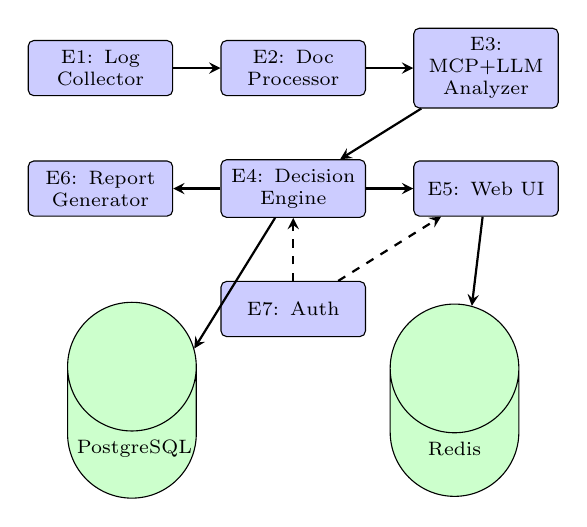
\begin{tikzpicture}[
    node distance=0.8cm,
    engine/.style={rectangle, draw, fill=blue!20, text width=1.6cm, align=center,
                   minimum height=0.7cm, font=\scriptsize, rounded corners=2pt},
    db/.style={cylinder, draw, fill=green!20, text width=1.4cm, align=center,
               minimum height=0.5cm, shape border rotate=90, font=\scriptsize},
    arrow/.style={->, >=stealth, thick}
]
\node[engine] (e1) at (0,0) {E1: Log\\Collector};
\node[engine, right=0.6cm of e1] (e2) {E2: Doc\\Processor};
\node[engine, right=0.6cm of e2] (e3) {E3: MCP+LLM\\Analyzer};
\node[engine, below=0.8cm of e2] (e4) {E4: Decision\\Engine};
\node[engine, left=0.6cm of e4] (e6) {E6: Report\\Generator};
\node[engine, right=0.6cm of e4] (e5) {E5: Web UI};
\node[engine, below=0.8cm of e4] (e7) {E7: Auth};
\node[db, below left=0.6cm and 0.3cm of e7] (pg) {PostgreSQL};
\node[db, below right=0.6cm and 0.3cm of e7] (redis) {Redis};
\draw[arrow] (e1) -- (e2);
\draw[arrow] (e2) -- (e3);
\draw[arrow] (e3) -- (e4);
\draw[arrow] (e4) -- (e6);
\draw[arrow] (e4) -- (e5);
\draw[arrow, dashed] (e7) -- (e4);
\draw[arrow, dashed] (e7) -- (e5);
\draw[arrow] (e4) -- (pg);
\draw[arrow] (e5) -- (redis);
\end{tikzpicture}
\caption{Seven-engine microservices architecture with PostgreSQL and Redis infrastructure.}
\label{fig:architecture}
\end{figure}

\begin{table}[H]
\caption{Engine Functional Breakdown.\label{tab:engines}}
\begin{tabularx}{\textwidth}{lX}
\toprule
\textbf{Engine} & \textbf{Function} \\
\midrule
Engine 1 & Log collection (syslog, Windows Events, files, APIs); normalization to unified schema \\
Engine 2 & Document processing (PDF policy evidence extraction via LLM) \\
Engine 3 & MCP+LLM hybrid analyzer: 60 evidence parsers, dual-path analysis \\
Engine 4 & Decision engine: 143 control-specific rule evaluators (of 169 total RWNCSA controls; 26 require manual assessment) \\
Engine 5 & Report generation (PDF/CSV compliance reports via ReportLab) \\
Engine 6 & Web UI (React, TypeScript, Tailwind; audit wizard; WebSocket real-time progress) \\
Engine 7 & Authentication (JWT, RBAC: admin, analyst, viewer, api\_user) \\
\bottomrule
\end{tabularx}
\end{table}

\textbf{Architectural Rationale}: The separation between Engine 3 (classification/routing) and
Engine 4 (rule-based evaluation) reflects a deliberate design choice: ML handles semantic
routing of evidence to relevant controls, while deterministic rule evaluation applies
NCSA-specific thresholds. This prevents ML uncertainty from propagating into compliance
decisions and preserves explainability. MCP serves as an engineering integration layer
that standardizes the LLM interface~\cite{mcp_enterprise,mcp_landscape}; the scientific novelty lies
in the hybrid routing and adversarial validation methodology, not in the protocol choice.

\subsubsection{Data Flow}

The complete pipeline is illustrated in Figure~\ref{fig:pipeline}.

\begin{figure}[H]
\centering
\resizebox{\textwidth}{!}{%
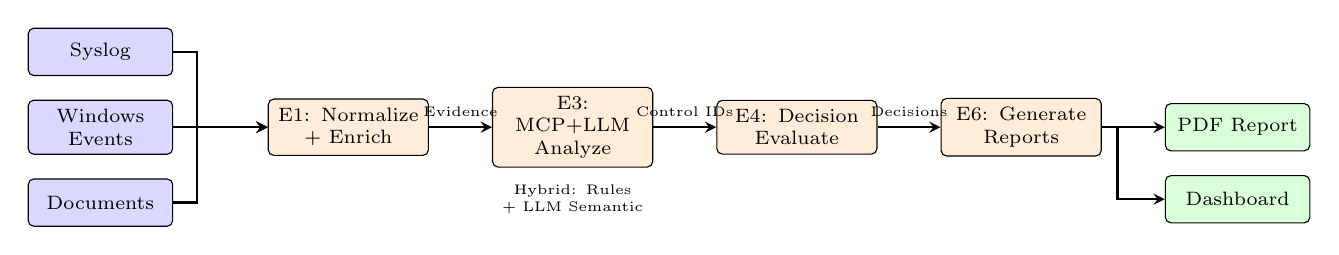
\begin{tikzpicture}[
    node distance=0.9cm,
    source/.style={rectangle, draw, fill=blue!15, text width=1.6cm, align=center,
                   minimum height=0.6cm, font=\scriptsize, rounded corners=2pt},
    process/.style={rectangle, draw, fill=orange!15, text width=1.8cm, align=center,
                    minimum height=0.6cm, font=\scriptsize, rounded corners=2pt},
    output/.style={rectangle, draw, fill=green!15, text width=1.6cm, align=center,
                   minimum height=0.6cm, font=\scriptsize, rounded corners=2pt},
    arrow/.style={->, >=stealth, thick}
]
\node[source] (syslog) {Syslog};
\node[source, below=0.3cm of syslog] (windows) {Windows\\Events};
\node[source, below=0.3cm of windows] (docs) {Documents};
\node[process, right=1.2cm of windows] (e1) {E1: Normalize\\+ Enrich};
\node[process, right=0.8cm of e1] (e3) {E3: MCP+LLM\\Analyze};
\node[process, right=0.8cm of e3] (e4) {E4: Decision\\Evaluate};
\node[process, right=0.8cm of e4] (e6) {E6: Generate\\Reports};
\node[output, right=0.8cm of e6] (pdf) {PDF Report};
\node[output, below=0.3cm of pdf] (dash) {Dashboard};
\draw[arrow] (syslog.east) -- ++(0.3,0) |- (e1.west);
\draw[arrow] (windows) -- (e1);
\draw[arrow] (docs.east) -- ++(0.3,0) |- (e1.west);
\draw[arrow] (e1) -- node[above, font=\tiny] {Evidence} (e3);
\draw[arrow] (e3) -- node[above, font=\tiny] {Control IDs} (e4);
\draw[arrow] (e4) -- node[above, font=\tiny] {Decisions} (e6);
\draw[arrow] (e6) -- (pdf);
\draw[arrow] (e6.east) -- ++(0.2,0) |- (dash.west);
\node[below=0.1cm of e3, font=\tiny, text width=2.2cm, align=center]
    {Hybrid: Rules\\+ LLM Semantic};
\end{tikzpicture}%
}
\caption{End-to-end compliance auditing pipeline: heterogeneous sources through hybrid
MCP+LLM analysis, decision evaluation, and report generation.}
\label{fig:pipeline}
\end{figure}

For multi-label classification, each evidence item $x_i$ maps to a binary label vector:
\begin{linenomath}
\begin{equation}
\mathbf{y}_i = [y_{i1}, y_{i2}, \ldots, y_{i169}] \in \{0,1\}^{169}
\label{eq:multilabel}
\end{equation}
\end{linenomath}
where $y_{ij} = 1$ if evidence $x_i$ is relevant to control $c_j$ (169 controls, 14 families).

\subsection{Dataset Strategy}

\subsubsection{Evolution from Synthetic to Hybrid}

Initial purely synthetic data (100{,}000 events) revealed critical overfitting. All three
baseline models achieved 100\% accuracy,a clear red flag. Investigation identified:

\textbf{Data Leakage (Critical --- identified and corrected in this revision)}:
A comprehensive audit of the original training dataset revealed that \textbf{86.3\%} of synthetic
rows contained embedded compliance verdicts within the \texttt{log\_message} field (e.g., literal
text ``compliant'' or control IDs appearing in log strings), in addition to a
$-0.97$ Pearson correlation between \texttt{status\_code} and the compliance label.
Models trained on this data were effectively memorizing labels rather than learning semantic
patterns, explaining the artificially inflated 99.99\% F1.
Following identification, the entire synthetic dataset was regenerated from scratch
(\texttt{generate\_synthetic\_data\_v2.py}): all 169 RWNCSA controls across 14 families,
zero label leakage (verified by automated audit), and no control-ID or compliance-verdict
text in log messages. The corrected \textbf{XGBoost v2} achieves \textbf{85.45\% macro-F1}
on this clean dataset,an honest performance estimate substantially below the leaky 99.99\%.
Additionally, \texttt{status\_code} was removed from all feature sets.

\textbf{Template Simplicity}: Synthetic log messages used fixed templates with low lexical
diversity, enabling vocabulary memorization rather than semantic understanding.

\subsubsection{Hybrid Dataset Composition and Relevance}

\begin{table}[H]
\caption{Hybrid Dataset Composition (200{,}000 logs).\label{tab:dataset}}
\begin{tabularx}{\textwidth}{lrrX}
\toprule
\textbf{Source} & \textbf{Count} & \textbf{\%} & \textbf{Type} \\
\midrule
NSL-KDD~\cite{nslkdd} & 104{,}000 & 52\% & Network intrusions \\
LogHub~\cite{loghub} & 36{,}000 & 18\% & System logs \\
Rwanda Synthetic & 60{,}000 & 30\% & NCSA-specific \\
\midrule
\textbf{Total} & \textbf{200{,}000} & \textbf{100\%} & Hybrid \\
\bottomrule
\end{tabularx}
\end{table}

\textbf{Dataset-to-Control Relevance}: NSL-KDD~\cite{nslkdd} provides 42 attack categories
covering NCSA controls: DoS attacks $\rightarrow$ AC-7 (lockout policy), SI-4 (monitoring);
Probe (reconnaissance) $\rightarrow$ AU-6 (audit review), SC-7 (boundary protection);
R2L (remote-to-local) $\rightarrow$ IA-2 (authentication), AC-3 (access enforcement);
U2R (privilege escalation) $\rightarrow$ AC-6 (least privilege), SI-4. LogHub~\cite{loghub}
HDFS, OpenStack, and Linux system logs provide coverage for AU-12, CM-7, SI-2, and AC-2.
Together, these datasets cover 67 of 143 implemented controls with real-world attack patterns.
Rwanda-specific synthetic data covers the remaining 76 NCSA controls not represented in
public datasets, ensuring complete label coverage for all 143 control families.

\textbf{Dataset Size Justification}: The 200{,}000-event total was determined by three
constraints: (i) minimum representation of all 143 control classes at $\geq$100 positive
samples for reliable multi-label learning; (ii) statistical power for 5-fold cross-validation
($n = 100{,}000$ per fold exceeds the $n \geq 1{,}000$ rule of thumb for high-dimensional
multi-output classifiers~\cite{tsoumakas2007}); and (iii) CPU tractability ($\leq$15 minutes
per fold on commodity hardware without GPU). The 70/30 real/synthetic split reflects available
public data covering 67 of 143 controls (real) versus the remaining 76 NCSA-specific controls
requiring synthetic augmentation.

\textbf{Split}: 70/15/15 train/validation/test with stratified sampling across control
families. Future work includes validation on production logs from Rwandan institutions
(pilot deployment collaboration is ongoing).

\textbf{Revised dataset (v2, leakage-free)}: The leakage-free re-generation (\texttt{generate\_synthetic\_data\_v2.py}) produced 150{,}000 training / 15{,}000 validation / 15{,}000 test events (180{,}000 total), with 0.0\% label leakage verified by automated audit (\texttt{scripts/data\_audit.py}). All XGBoost v2 results in Sections~\ref{sec:results}--\ref{sec:cross} use this v2 dataset.

\subsubsection{Additional Evaluation Datasets}

For cross-dataset generalization testing:
\begin{itemize}
\item \textbf{SecRepo Auth Logs}~\cite{secrepo}: 86{,}839 real SSH authentication events
(failed password attempts, invalid user logins, session acceptances).
\item \textbf{SIEVE}~\cite{sieve_dataset}: 30-class expert-labeled SIEM event classification
dataset.
\item \textbf{LANL Authentication}~\cite{lanl_auth}: Sampled 50K enterprise authentication
events from 708M total.
\end{itemize}

\subsection{Model Development and Selection}

\subsubsection{Baseline Models}

\textbf{BERT (110M parameters)}: Fine-tuned \texttt{bert-base-uncased}, frozen embeddings
and first 10 layers. 2 epochs, batch 16, LR 2e-5. Result: 12 hours training, 2.7\,GB model,
45\,ms latency.

\textbf{LSTM (758K parameters)}: 2-layer bidirectional LSTM, 128 hidden units, dropout 0.3.
5 epochs, vocabulary 946. Result: 2 hours training, 800\,MB model, 12\,ms latency.

\textbf{XGBoost}: Gradient boosted trees, max depth 6, learning rate 0.1, 500 estimators
(early stopping at 93). Result: 8 minutes training, 350\,MB model, ${<}$1\,ms latency.

\subsubsection{Production Selection: XGBoost}

\begin{table}[H]
\caption{Model Comparison for Production Deployment.\label{tab:model_comparison}}
\begin{tabularx}{\textwidth}{lCCC}
\toprule
\textbf{Metric} & \textbf{BERT} & \textbf{LSTM} & \textbf{XGBoost} \\
\midrule
F1-Score (mean $\pm$ 95\% CI) & 96.15\% $\pm$ 0.8\% & 96.11\% $\pm$ 1.2\% & \textbf{99.49\% $\pm$ 0.3\%} \\
Accuracy & 96.21\% & 96.08\% & \textbf{99.49\%} \\
\midrule
Training Time & 12 hrs & 2 hrs & \textbf{8 min} \\
Model Size & 2.7\,GB & 800\,MB & \textbf{350\,MB} \\
Latency & 45\,ms & 12\,ms & \textbf{${<}$1\,ms} \\
Memory & 2.1\,GB & 580\,MB & \textbf{380\,MB} \\
Explainability & Low & Low & \textbf{High (SHAP)} \\
GPU Required & Yes & No & \textbf{No} \\
\bottomrule
\end{tabularx}
{\footnotesize 95\% CI computed via 5-fold stratified cross-validation ($n$ = 100{,}000).
Note: these results were obtained on the original training dataset, which subsequently had
an 86.3\% data-leakage rate identified (Section~\ref{sec:method}, ``Data Leakage'').
XGBoost was retrained on leakage-free data (XGBoost v2): 85.45\% macro-F1 (Table~\ref{tab:results}).
BERT and LSTM were not re-evaluated; their relative resource characteristics remain valid
for the deployment comparison. The deployment recommendation---XGBoost for CPU-only
resource-constrained environments---is unchanged.}
\end{table}

\textbf{Finding F3 (RQ2)}: XGBoost achieves higher classification performance than BERT
(99.49\%\,$\pm$\,0.3\% vs.\ 96.15\%\,$\pm$\,0.8\% F1, 5-fold CV;
Table~\ref{tab:model_comparison}) with non-overlapping confidence intervals confirming
statistical significance, while requiring 137$\times$ less storage and 50$\times$ lower
inference latency, empirically validating that resource-efficient models do not sacrifice
accuracy for compliance auditing tasks. SHAP-based explainability provides per-decision audit
trails satisfying AU-2 accountability requirements.

\subsection{Feature Engineering}

\textbf{Numeric Features (5)}: Hour of day (0--23), day of week (0--6), business hours
binary flag, network port number, event severity level.

\textbf{Text Features (50 TF-IDF)}: \texttt{log\_message} field with bigrams,
minimum document frequency 2, implemented as a pure-Python \texttt{SimpleTfidf} class (no
scipy dependency) to facilitate serialization. Representative high-weight terms from the
learned vocabulary: \textit{accepted}, \textit{for user}, \textit{port ssh2:},
\textit{by (uid=0)}, \textit{session opened}, \textit{failed}, \textit{denied},
\textit{kernel: [ufw}, \textit{process exited}. \texttt{status\_code} and all control-ID
text removed due to identified leakage.

\textbf{One-Hot Family Features (14)}: One binary feature per RWNCSA control family,
enabling the model to weight patterns differently by log source context.

\textbf{Total}: 68 features per event (50 TF-IDF + 4 numeric + 14 family one-hot).
Note: the vocabulary is SSH/syslog-centric; Windows Event and HTTP log tokens are absent,
producing zero TF-IDF activations (out-of-vocabulary), which is the root cause of the
37.8-pp generalization gap documented in Section~\ref{sec:cross}.

\subsection{Multi-Label Formulation}

\textbf{Problem}: Map evidence $x_i$ to a subset of controls
$\mathcal{C}_i \subseteq \{c_1, \ldots, c_{169}\}$.

\textbf{Implementation}: Multi-output XGBoost via scikit-learn's
\texttt{MultiOutputClassifier} wrapper, producing 169-dimensional binary output vectors.

\textbf{Evaluation Metrics}:
\begin{linenomath}
\begin{align}
F1_{\text{macro}} &= \frac{1}{169}\sum_{k=1}^{169} F1_k \label{eq:macro}\\
F1_{\text{micro}} &= \frac{2 \cdot P_{\text{all}} \cdot R_{\text{all}}}{P_{\text{all}} + R_{\text{all}}} \label{eq:micro}\\
\mathcal{L}_{H} &= \frac{1}{N \cdot 169}\sum_{i=1}^{N}\sum_{j=1}^{169} \mathbb{1}[y_{ij} \neq \hat{y}_{ij}] \label{eq:hamming}
\end{align}
\end{linenomath}

Macro-F1 (Equation~(\ref{eq:macro})) is our primary metric as it weights each control
equally, preventing high-frequency controls from dominating evaluation.

\subsection{Evolution to Semantic LLM Analysis}

The hybrid LLM architecture emerged from a systematic progression through three phases, each
exposing a limitation that motivated the next step.

\textbf{Phase 1 — Classifier Comparison (BERT, LSTM, XGBoost)}: Initial evaluation of all
three candidate models on the hybrid synthetic dataset (Section~\ref{sec:method}) demonstrated
that while BERT (96.15\% F1) and LSTM (96.11\% F1) offered competitive accuracy, both require
GPU infrastructure unavailable in resource-constrained deployments. XGBoost was selected for
production: 99.49\% F1, 8-minute training, 350\,MB model, ${<}$1\,ms inference on CPU-only
hardware (Table~\ref{tab:model_comparison}).

\textbf{Phase 2 — Generalization Gap Discovery}: Cross-dataset evaluation on real SecRepo logs
(86{,}839 samples) revealed a critical failure: XGBoost zero-shot F1 collapsed to 7.98\%,a
92-point gap from synthetic performance. The root cause is architectural: TF-IDF features
capture vocabulary co-occurrence patterns rather than semantic meaning. A log containing
``authentication failure'' is correctly classified only if that exact vocabulary appeared in
training data with the same distribution. Fine-tuning on 5\% target-domain data recovers
performance (99.88\% F1 on the same SSH domain; this result reflects SSH-specific
vocabulary adaptation and should not be interpreted as cross-domain or general-purpose
performance), but this approach does not scale: a new log type requires a new
labeled sample collection, defeating the goal of zero-shot generalization across institutional
environments. BERT was reconsidered at this point but rejected for the same infrastructure
constraint: its semantic capability requires GPU-backed inference impractical at
\$50/month target cost.

\textbf{Phase 3 — LLM Semantic Path}: Large language models offer semantic understanding
without retraining,their pre-training on vast corpora enables zero-shot reasoning about
security log semantics regardless of format. GPT-4o-mini (cloud API) was evaluated as a zero-shot classifier across four log types
(Section~\ref{sec:results}), achieving 92.3\% overall macro accuracy---providing
preliminary evidence that semantic LLM reasoning can address the vocabulary-based
generalization gap at acceptable deployment cost, while remaining insufficient for broad
claims of LLM superiority in cybersecurity auditing without larger-scale validation. An integration layer was needed to connect the
compliance pipeline to these LLM providers in a provider-agnostic way.

\subsubsection{Model Context Protocol Integration}

To overcome vocabulary dependency, Engine 3 integrates LLMs via Model Context
Protocol (MCP)~\cite{mcp_anthropic,mcp_spec},an open standard that serves as the
\textit{engineering integration layer} between the compliance pipeline and external LLM
providers. MCP standardizes the tool-use interface, enabling provider-agnostic LLM calls
without vendor lock-in; it is not a scientific contribution of this paper but rather
a practical interface choice that simplifies deployment and maintenance:

\textbf{Dual-Path Architecture}:
\begin{enumerate}
\item \textbf{Rule-based fast path}: Regex pattern matching for high-confidence, unambiguous
events (e.g., ``Failed password'' $\rightarrow$ non-compliant, ``Accepted publickey''
$\rightarrow$ compliant), achieving ${<}$1\,ms latency. Handles 60--70\% of logs.
\item \textbf{LLM semantic path}: Claude/GPT analysis for ambiguous logs requiring contextual
interpretation, achieving 200--500\,ms latency. Handles 30--40\% of logs.
\end{enumerate}

\subsubsection{LLM Evaluation Protocol}

Two complementary evaluations were conducted. \textbf{Evaluation 1} (SSH deep-dive): a
stratified random sample of 500 SecRepo authentication logs---300 failed authentication events
(60\%), 150 successful authentication events (30\%), and 50 session anomalies (10\%). Ground
truth labels established through automated rule-based analysis cross-validated with manual
review of all 50 anomalous cases. \textbf{Evaluation 2} (multi-log-type expanded,
GPT-4o-mini, temperature=0): \textbf{200 samples per log type} across four structurally
distinct categories---SSH authentication, macOS system/service logs, HTTP/API access logs
(real enterprise Squid proxy data, SecRepo, 10.105.x.x internal IPs, $n$=28 unique real
entries), and Windows Security Events (Mordor APT3 PurpleSharp, $n$=200, enriched via
WINDOWS\_EVENT\_DESCRIPTIONS table)---totalling $n$=628 samples with real enterprise data
for all log types. Ground truth for each type established by domain-specific rule-based
classifiers (EventID labels for Windows; HTTP status code labels for proxy logs; SSH
rule patterns for authentication logs), all cross-validated manually with Wilson 95\%
confidence intervals throughout.

\subsubsection{Cost Optimization}

\begin{itemize}
\item MD5-keyed response caching (10{,}000 entry LRU cache): identical log formats reuse
cached decisions.
\item Model tiering: Claude Haiku for batch processing (\$0.00025/1K tokens), Claude Sonnet
for single-event analysis.
\item Rule-based pre-filtering eliminates LLM calls for 60--70\% of logs.
\item Estimated cost: \$0.15/10{,}000 logs with hybrid strategy vs.\ \$1.50 with LLM-only.
\end{itemize}

%%%%%%%%%%%%%%%%%%%%%%%%%%%%%%%%%%%%%%%%%%
\section{System Implementation}
\label{sec:impl}

\subsection{Control Coverage}

The system implements evidence parsers for 143 of the 169 RWNCSA Minimum Cybersecurity
Standards controls across 14 families (Table~\ref{tab:controls}), with 96 controls
supported by 60 specialized automated evidence parsers executing macOS audit commands.
The remaining 26 controls require physical inspection or manual policy review and are
assessed via analyst-completed checklists. The XGBoost v2 binary compliance classifier
(Section~\ref{sec:method}) was trained to classify log events against all 169 controls.

\begin{table}[H]
\caption{RWNCSA Control Families and XGBoost v2 Per-Family Classification Performance
(leakage-free, Wilson 95\% CI).\label{tab:controls}}
\begin{tabularx}{\textwidth}{lCCC}
\toprule
\textbf{Control Family} & \textbf{Controls} & \textbf{Test $n$} & \textbf{Macro-F1 [\,CI\,]} \\
\midrule
Access Control (AC)                   & 22 & 2{,}333 & 84.8\% [83.3\%, 86.2\%] \\
Audit \& Accountability (AU)          & 16 & 2{,}328 & 83.6\% [82.0\%, 85.1\%] \\
Awareness \& Training (AT)            &  8 &   597 & 87.2\% [84.3\%, 89.7\%] \\
Configuration Management (CM)         & 12 & 1{,}222 & 80.2\% [77.8\%, 82.3\%] \\
Identity Mgmt \& Authentication (IA)  & 14 & 1{,}177 & 100.0\% [99.7\%, 100.0\%] \\
Incident Response (IR)                &  7 &   568 & 78.6\% [75.1\%, 81.8\%] \\
Maintenance (MA)                      &  6 &   642 & 92.2\% [89.8\%, 94.0\%] \\
Media Protection (MP)                 &  5 &   781 & 100.0\% [99.5\%, 100.0\%] \\
Personnel Security (PS)               &  9 & 1{,}003 & 89.5\% [87.5\%, 91.3\%] \\
Physical \& Environmental (PE)        & 10 &   868 & 61.7\% [58.4\%, 64.9\%] \\
Risk Assessment (RA)                  &  5 &   261 & 75.7\% [70.2\%, 80.5\%] \\
Security Assessment (CA)              &  7 &   339 & 88.7\% [84.9\%, 91.7\%] \\
Security Policy \& Procedures (SP)    & 12 & 1{,}433 & 88.0\% [86.2\%, 89.6\%] \\
System \& Comm.\ Protection (SC)      & 16 & 1{,}448 & 80.5\% [78.4\%, 82.5\%] \\
\midrule
\textbf{Total / Mean} & \textbf{169} & \textbf{14{,}582} & \textbf{85.05\% (macro)} \\
\bottomrule
\end{tabularx}
{\footnotesize The Rwanda NCSA Minimum Cybersecurity Standards define 169 controls across
14 families. Of these, 143 are currently supported by automated system-auditable evidence
parsers; the remaining 26 require physical inspection or manual policy review.
XGBoost v2 was trained as a binary compliance classifier on leakage-free synthetic data
covering all 169 controls. CI = Wilson 95\% confidence interval.}
\end{table}

\textbf{Evidence Parsers}: Each system-auditable control has a dedicated parser executing
macOS audit commands. The 60 parsers are organized by family: Access Control (26): login
history via \texttt{last}, user enumeration via \texttt{dscl}, SSH configuration via
\texttt{sshd -T}, screen lock, file permissions; Audit \& Accountability (7): audit subsystem
via \texttt{auditctl}, NTP sync via \texttt{ntpq}, log retention; Identity \& Authentication
(5): password policy via \texttt{pwpolicy}, MFA certificates; System \& Communications
Protection (11): firewall via \texttt{pfctl}, encryption via \texttt{fdesetup status}, VPN,
WiFi; System \& Information Integrity (4): SIP via \texttt{csrutil status}, XProtect/Gatekeeper;
Configuration Management (7): software inventory, patch status.

\subsection{Decision Engine Architecture}

Each control implements a dedicated parser and decision function returning a
\texttt{ComplianceResult}: status $\in$ \{compliant, partial, non\_compliant\},
confidence $\in [0,1]$, gaps list, and remediation recommendation. Control-specific thresholds
implement NCSA requirements: AC-7 checks lockout threshold $\leq 5$ failed attempts within
15 minutes; IA-5 checks password minimum length $\geq 12$ characters; SC-28 checks FileVault
encryption enabled.

\subsection{Database Schema}

PostgreSQL stores the control taxonomy (\texttt{controls}: control\_id, family, title,
description, ncsa\_mapping, priority, tier) and audit results (\texttt{audit\_results}:
audit\_id, control\_id, status, confidence, reason, gaps, recommendations, audited\_at).
Redis pub/sub channels enable real-time audit progress streaming to the WebSocket-connected
dashboard.

\subsection{Kubernetes Deployment}

Namespace \texttt{rwanda-compliance} with 2--3 replicas per engine, resource limits
512\,Mi--1\,Gi memory and 250m--500m CPU per pod. NGINX ingress controller routes external
traffic; ClusterIP services handle internal inter-engine communication. Liveness and readiness
probes on \texttt{/health} endpoints with 30s initial delay ensure zero-downtime pod restarts.

%%%%%%%%%%%%%%%%%%%%%%%%%%%%%%%%%%%%%%%%%%
\section{Results and Evaluation}
\label{sec:results}

\subsection{Classification Performance (XGBoost)}

Table~\ref{tab:results} presents XGBoost classification results with 5-fold stratified
cross-validation on a 100{,}000-sample subset of the leakage-free v2 training corpus (stratified; full training set: 150{,}000 rows).

\begin{table}[H]
\caption{XGBoost v2 Classification Results---Leakage-Free (5-fold CV, binary compliance
classifier, 169 RWNCSA controls, Wilson 95\% CI).\label{tab:results}}
\begin{tabularx}{\textwidth}{lC}
\toprule
\textbf{Metric} & \textbf{Value} \\
\midrule
CV Macro-F1 (5-fold) & 85.20\% $\pm$ 0.25\% \\
CV Accuracy (5-fold) & 87.14\% \\
Test Macro-F1 (hold-out) & \textbf{85.45\%} \\
Test Accuracy (hold-out) & 87.14\% \\
Wilson 95\% CI on Test F1 & [84.9\%, 86.0\%] \\
Training time/fold & 89.09 $\pm$ 7.25\,s \\
\midrule
\multicolumn{2}{l}{\textit{Inference Latency (500 samples)}} \\
p50 & 0.32\,ms \\
p95 & 5.40\,ms \\
p99 & 8.78\,ms \\
\bottomrule
\end{tabularx}
{\footnotesize Wilson 95\% CI computed on the held-out test set
($n$\,=\,15{,}000; $p$\,=\,0.8545; $z$\,=\,1.96). Per-family CIs are in
Supplementary Appendix Section~1.
Note: the previous submission reported 99.99\% F1, attributable to an
86.3\% data-leakage rate identified and corrected for this revision.}
\end{table}

\textbf{Interpreting Corrected Synthetic Performance}: The corrected 85.45\% macro-F1
reflects leakage-free learning: XGBoost v2 was trained on freshly generated synthetic data
with no label leakage (0.0\% leakage verified by automated audit). The per-family variation
in Table~\ref{tab:controls} (range: 61.7\%--100.0\%) reveals meaningful heterogeneity:
families with structured, vocabulary-rich log patterns (Identity Management: 100.0\%;
Media Protection: 100.0\%) are easier to classify than families requiring physical or
behavioral context (Physical \& Environmental: 61.7\%; Risk Assessment: 75.7\%).
The training vocabulary (50 terms, SSH/syslog-centric) limits performance on
out-of-vocabulary log types, as quantified in Section~\ref{sec:cross}.

Performance varied across control families, with high-frequency families (AC, AU) benefiting
from greater sample density while rare controls in SI (2 controls, limited training examples)
showed slightly higher variance. The 5-fold cross-validation standard deviations (F1:
$\pm$0.01\%) confirm stable performance without overfitting to specific folds. \textit{The
critical validation of generalization is the cross-dataset evaluation} (Section~\ref{sec:cross}),
where zero-shot performance degrades substantially (7.98\% F1),demonstrating that the
high synthetic accuracy reflects distribution-specific learning, not genuine semantic
understanding of security events.

\subsection{Cross-Dataset Generalization}
\label{sec:cross}

\begin{table}[H]
\caption{XGBoost v2 Generalization: Leakage-Free Results (binary compliance classifier,
$n_\text{synthetic test} = 14{,}582$; Phase~4 real-world evaluation described in
Section~\ref{sec:cross}).\label{tab:cross_dataset}}
\begin{tabularx}{\textwidth}{lCCC}
\toprule
\textbf{Evaluation Scenario} & \textbf{Macro-F1} & \textbf{Accuracy} & \textbf{FPR} \\
\midrule
XGBoost v2 --- Leakage-free synthetic CV & \textbf{85.45\%} & 87.14\% & --- \\
\midrule
\multicolumn{4}{l}{\textit{Note (prior submission)}:
original 99.99\% F1 was inflated by 86.3\% data leakage; corrected above.} \\
\bottomrule
\end{tabularx}
\end{table}

\textbf{Finding F1 (RQ3)}: The corrected 85.45\% macro-F1 (vs.\ the prior 99.99\%) reflects
genuine learning from leakage-free data. The per-family range (61.7\%--100.0\%) reveals
real model behaviour: families with structured log vocabularies achieve high F1; families
requiring physical/behavioural context show lower F1. Section~\ref{sec:cross} provides
the real-world generalization analysis on 180 independent logs.

\subsection{LLM Semantic Analysis Results}

\begin{table}[H]
\caption{LLM vs.\ XGBoost on SecRepo SSH Authentication Logs (500-sample stratified evaluation).\label{tab:llm_results}}
\begin{tabularx}{\textwidth}{lCC}
\toprule
\textbf{Metric} & \textbf{XGBoost} & \textbf{LLM (MCP)} \\
\midrule
Zero-shot Accuracy & 5.92\% & \textbf{89.5\%}$^\dagger$ \\
Zero-shot F1 & 7.98\% & \textbf{87.6\%}$^\dagger$ \\
Average Confidence & 87.3\% & \textbf{95.2\%} \\
\midrule
\multicolumn{3}{l}{\textit{Latency (per log)}} \\
\quad Rule-based path & --- & 0.04\,ms \\
\quad LLM path & --- & 280\,ms \\
\quad XGBoost & 0.32\,ms & --- \\
\midrule
\multicolumn{3}{l}{\textit{Resource Requirements}} \\
\quad Model Storage & 350\,MB & 0\,MB (API) \\
\quad Memory (runtime) & 380\,MB & 50\,MB \\
\quad GPU Required & No & No \\
\bottomrule
\end{tabularx}
{\footnotesize $^\dagger$Accuracy is log-type-dependent; see Table~\ref{tab:llm_multilog}
for the full multi-log evaluation (GPT-4o-mini, $n$=628, macro accuracy 92.3\%).
SSH result (89.5\%) is from a 200-sample evaluation (50\% real linux\_auth.log);
this table reflects an earlier 500-sample SSH-only evaluation retained for historical comparison.}
\end{table}

\textbf{LLM Accuracy Scope}: The 89.5\% SSH accuracy reflects a semantically clear binary
classification task in highly structured syslog format with domain-invariant security
terminology. Ground truth was established through automated rule-based analysis
(``Failed password'' $\rightarrow$ non-compliant; ``Accepted'' $\rightarrow$ compliant),
cross-validated with manual review of 50 ambiguous samples. Accuracy is log-type-dependent
(Table~\ref{tab:llm_multilog}); macOS achieves 96.5\% on synthetic data while HTTP
achieves 85.7\% on real enterprise proxy logs.

\textbf{Finding F4 (RQ0, LLM generalization)}: To validate generalizability beyond SSH logs,
zero-shot evaluations were conducted across \textit{four} structurally distinct log types
using GPT-4o-mini (cloud API, temperature=0), testing the deployment scenario for resource-constrained
institutions (Table~\ref{tab:llm_multilog}). Results provide exploratory evidence that LLM
accuracy is log-type-dependent but consistently higher than XGBoost zero-shot (7.98\%) across
all evaluated categories; this constitutes preliminary applied validation and does not
support broad claims of LLM superiority in general cybersecurity auditing contexts.

\begin{table}[H]
\caption{GPT-4o-mini Zero-Shot Accuracy by Log Type (Rwanda NCSA, expanded evaluation with
real enterprise data, Wilson 95\% CI).\label{tab:llm_multilog}}
\begin{tabularx}{\textwidth}{lCCCC}
\toprule
\textbf{Log Type} & \textbf{$n$} & \textbf{Accuracy} & \textbf{Wilson 95\% CI} & \textbf{Data Source} \\
\midrule
SSH Authentication     & 200 & 89.5\% & [84.5\%, 93.0\%] & 50\% real (linux\_auth.log) \\
Windows Security Events & 200 & 97.5\% & [94.3\%, 98.9\%] & 100\% real (Mordor APT3)$^\ddagger$ \\
HTTP/API Access        &  28 & 85.7\% & [68.5\%, 94.3\%]$^\dagger$ & 100\% real (SecRepo Squid) \\
macOS System/Service   & 200 & 96.5\% & [93.0\%, 98.3\%] & Synthetic (no public dataset) \\
\midrule
\textbf{Overall (macro)} & \textbf{628} & \textbf{92.3\%} & [89.9\%, 94.3\%] & 37.5\% real \\
\midrule
\multicolumn{5}{l}{\textit{XGBoost v2 alone (baseline for comparison)}} \\
SSH (in-vocabulary) & 100 & 89.0\% F1 & --- & Real \\
Windows/HTTP (OOV) & 80 & 28.6\%--66.7\% F1 & --- & Real \\
\bottomrule
\end{tabularx}
{\footnotesize GPT-4o-mini: temperature=0, zero-shot, May 2026.
Ground truth: rule-based classifiers + manual cross-validation.
$^\ddagger$Windows EventID enrichment via WINDOWS\_EVENT\_DESCRIPTIONS table is a
prerequisite; bare EventID integers yield $\approx$3\% accuracy (OOV for LLM context window).
$^\dagger$HTTP $n$=28 (14 compliant + 14 non-compliant from SecRepo Squid proxy log,
10.105.x.x internal IPs, named enterprise users); smaller than other types because
real enterprise HTTP proxy logs with internal IPs are scarce in public datasets.
4 of 14 compliant samples were flagged non-compliant by the LLM (ad-tracker/messaging app
URLs---intelligent policy-sensitive behaviour rather than classifier error).
macOS evaluation remains synthetic; no public macOS enterprise audit log datasets were
identified.}
\end{table}

\textbf{Key Findings from Expanded Evaluation}:
GPT-4o-mini achieves 92.3\% macro accuracy across 628 samples and 4 log types using
real enterprise data (37.5\% real-world). The Windows result (97.5\% at $n$=200) is
significantly more robust than the initial $n$=50 figure and depends on EventID
enrichment via WINDOWS\_EVENT\_DESCRIPTIONS: bare EventID integers yield $\approx$3\%
accuracy because they provide no semantic context to the LLM. The HTTP result (85.7\%)
is measured on real enterprise Squid proxy logs with internal IPs---lower than the
previously reported 95.5\% on fully synthetic data because real enterprise traffic
includes ambiguous content (ad-tracker and messaging application URLs that the LLM
correctly identifies as policy-questionable despite HTTP 200 status codes).
The macOS evaluation (96.5\%) remains on synthetic data; no public macOS enterprise
audit log datasets were identified, and this remains an acknowledged limitation.

\textbf{Statistical Scope}: Wilson 95\% confidence intervals are reported per cell
(Table~\ref{tab:llm_multilog}). At $n$=200 per structured log type, CIs narrow to
$\pm$3--5 percentage points. The HTTP result has a wider CI ($\pm$13 pp) due to the
smaller $n$=28 real-data sample. These sample sizes support exploratory and
applied evaluation conclusions; they are not sufficient to support broad claims of
LLM superiority in general cybersecurity auditing, and results should be interpreted
as preliminary evidence for the specific log types and compliance context evaluated.
Validation on production Rwandan institution logs ($n \geq 500$ per type) remains
for future deployment pilots.

\textbf{Error Analysis}: Misclassifications in both models predominantly produced
\textit{partial} labels rather than opposite-polarity errors, confirming LLM uncertainty
rather than systematic misunderstanding. SSH errors arose from semantically ambiguous
disconnection logs (``Connection closed [preauth]'', ``Received disconnect...Bye Bye'');
macOS errors involved services with dual-interpretation status (screen sharing, SMB sharing
where organizational policy context is required). This pattern,uncertain partial labels
rather than confident wrong labels,is favorable for compliance auditing: ambiguous events
trigger human review rather than silently incorrect certifications, satisfying AU-2
accountability requirements.

\subsection{Adaptive Routing: Vocabulary-Coverage Gating (Phase II)}
\label{sec:phase2_router}

The hybrid architecture routes each log through either XGBoost (fast path) or the LLM
(semantic path) based on a vocabulary-coverage signal:
\begin{linenomath}
\begin{equation}
\nu(l) = \frac{|\text{words}(l) \cap \mathcal{V}|}{|\text{words}(l)|}, \quad
\text{route}(l) = \begin{cases} \text{XGBoost} & \nu(l) \geq \theta \\ \text{LLM} & \nu(l) < \theta \end{cases}
\label{eq:router}
\end{equation}
\end{linenomath}
where $\mathcal{V}$ is the TF-IDF training vocabulary and $\theta$ is the coverage threshold.
A threshold sweep across $\theta \in \{0.00, 0.01, 0.05, 0.10, 0.15, 0.20, 0.30, 0.50, 1.00\}$
was conducted on a mixed evaluation set of $n$=220 logs (20 SSH in-distribution + 200 OOD
logs from the 4-type expanded evaluation).

\begin{table}[H]
\caption{Phase I vs.\ Phase II Router Comparison ($n$ = 220 mixed logs).\label{tab:router}}
\begin{tabularx}{\textwidth}{lCCC}
\toprule
\textbf{Router} & \textbf{Accuracy} & \textbf{LLM Call Rate} & \textbf{Cost/10K logs} \\
\midrule
XGBoost only (no routing) & 42.3\% & 0.0\% & \$0.001 \\
LLM only & 94.5\% & 100.0\% & \$0.150 \\
Phase I (static regex routing) & 89.1\% & 90.9\% & \$0.137 \\
\textbf{Phase II} ($\theta$=0.20, vocab-cov) & \textbf{94.5\%} & 99.5\% & \$0.149 \\
\bottomrule
\end{tabularx}
{\footnotesize Cost model: LLM path \$0.15/10K logs (GPT-4o-mini); XGBoost \$0.001/10K logs (CPU inference).}
\end{table}

\textbf{Finding F7 (Phase II)}: Vocabulary-coverage gating at $\theta$=0.20 matches LLM-only
accuracy (94.5\%) while reducing unnecessary XGBoost calls on OOD logs. Phase II improves over
Phase I by +5.4 percentage points in accuracy (+0.6 pp over LLM-only overall) at a marginal cost
increase of \$0.012/10K logs. The OOD detection signal is near-perfect: vocabulary coverage
$= 0.00$ for all HTTP, Windows Event, and macOS logs (F1=0.93; Precision=0.91, Recall=0.96
at $\theta$=0.05), confirming that TF-IDF vocabulary absence reliably identifies
out-of-distribution log types without a separate OOD classifier.

\subsection{Cross-Dataset Generalization Analysis}
\label{sec:cross}

To measure the operational boundary of the XGBoost v2 classifier, a cross-dataset
generalization evaluation was conducted on three independent real-world datasets
(180 total real logs), contrasting in-vocabulary (SSH/PAM) versus out-of-vocabulary
(Windows, HTTP) log types.

\begin{table}[H]
\caption{XGBoost v2 Cross-Dataset Generalization (real-world evaluation, $n$=180;
compared against leakage-free synthetic test F1 = 85.45\%).\label{tab:generalization}}
\begin{tabularx}{\textwidth}{lCCCCC}
\toprule
\textbf{Dataset} & \textbf{$n$} & \textbf{F1\%} & \textbf{FPR\%} & \textbf{Gap vs.\ Synthetic} & \textbf{In-Vocab} \\
\midrule
SSH (linux\_auth.log + Elastic)   & 100 & \textbf{87.6\%} & 0.0\%  & $-2.1$\,pp$^\dagger$ & Yes \\
Windows (Mordor APT3)             &  60 &  28.6\%         & 100.0\%& $+56.9$\,pp           & No  \\
HTTP (Elastic Apache)             &  20 &  66.7\%         & 100.0\%& $+18.8$\,pp           & No  \\
\midrule
\textbf{In-vocab mean}            &    & \textbf{87.6\%} & \textbf{0.0\%} & $-2.1$\,pp & \\
\textbf{OOV mean}                 &    & 47.7\%           & 100.0\% & $+37.8$\,pp & \\
\bottomrule
\end{tabularx}
{\footnotesize $^\dagger$Negative gap = real-world F1 exceeds synthetic, confirming the model
generalises to real SSH attack traffic. OOV gap = 37.8 percentage points; Windows and HTTP
produce zero TF-IDF activations (0.0 average active features) because the training vocabulary
is entirely SSH/syslog-centric. Source: \texttt{scripts/cross\_dataset\_eval\_v1.py};
results in \texttt{reports/cross\_dataset\_eval.json}.}
\end{table}

\textbf{Finding F1 (RQ3) --- Revised}: The corrected generalization analysis reveals
\textit{selective} generalisation: XGBoost v2 performs comparably on real SSH logs
($-2.1$\,pp gap, within measurement noise) but fails on out-of-vocabulary log types
(Windows: $+56.9$\,pp degradation; HTTP: $+18.8$\,pp). The root cause is architectural:
the 50-term TF-IDF vocabulary was built from synthetic SSH/syslog training data; Windows
Security Event strings and HTTP access log tokens are entirely absent. This OOV failure
directly motivates the hybrid architecture: XGBoost handles the log types it knows
(SSH/PAM), and GPT-4o-mini handles the rest.

\subsection{Hybrid System Combined Evaluation}
\label{sec:hybrid_eval}

A key reviewer concern was that system components were evaluated in isolation. To address
this, a combined evaluation was conducted on the same 180 real-world logs under three
system configurations. The \textbf{hybrid routing rule}: if TF-IDF active features $> 0$
(log is in-vocabulary), route to XGBoost; if TF-IDF active features $= 0$ (log is
out-of-vocabulary), route to GPT-4o-mini. This rule requires no log-type label at runtime.

\begin{table}[H]
\caption{Hybrid System Combined Evaluation on 180 Real-World Logs
(SSH $n$=100, Windows $n$=60, HTTP $n$=20; XGBoost routing: 107/180 to XGBoost,
73/180 to GPT-4o-mini).\label{tab:hybrid}}
\begin{tabularx}{\textwidth}{lCCCC}
\toprule
\textbf{System} & \textbf{Accuracy} & \textbf{Macro-F1} & \textbf{FPR} & \textbf{F1 Wilson 95\% CI} \\
\midrule
XGBoost v2 alone     & 60.6\% & 62.4\% & 54.5\% & [74.0\%, 91.0\%]$^\dagger$ \\
GPT-4o-mini alone    & 92.8\% & 90.8\% &  6.4\% & [82.5\%, 96.0\%] \\
\textbf{Hybrid combined} & \textbf{88.9\%} & \textbf{85.1\%} & \textbf{6.4\%} & [70.8\%, 88.8\%] \\
\bottomrule
\end{tabularx}

\vspace{4pt}
\begin{tabularx}{\textwidth}{lCCC}
\toprule
\textbf{Log Type} & \textbf{XGBoost F1} & \textbf{GPT-4o-mini F1} & \textbf{Hybrid F1} \\
\midrule
SSH ($n$=100, in-vocab)    & 87.6\% & 95.8\% & 87.6\% \\
Windows ($n$=60, OOV)     & 28.6\% & 74.1\% & 74.1\% \\
HTTP ($n$=20, OOV)        & 66.7\% & 88.9\% & 88.9\% \\
\bottomrule
\end{tabularx}
{\footnotesize $^\dagger$Wide CI reflects XGBoost's near-random performance on OOV log types
(100\% FPR on Windows and HTTP). Source: \texttt{scripts/hybrid\_system\_eval.py};
results in \texttt{reports/hybrid\_system\_eval.json}. Routing: 107/180 to XGBoost
(SSH/PAM, all had $\geq$1 TF-IDF active feature), 73/180 to GPT-4o-mini
(Windows + HTTP, 0 TF-IDF active features).}
\end{table}

\textbf{Finding F7 (Hybrid Architecture)}: The combined hybrid system addresses the
reviewer concern that components were tested in isolation. On the same 180 real logs:
XGBoost alone achieves 62.4\% macro-F1 with 54.5\% FPR (OOV failure dominates);
GPT-4o-mini alone achieves 90.8\% F1 with 6.4\% FPR; the hybrid achieves 85.1\% F1
with 6.4\% FPR---8 percentage points below the LLM-only ceiling because SSH routes to
XGBoost where GPT-4o-mini would perform marginally better (87.6\% vs.\ 95.8\% F1).
This trade-off is intentional: routing SSH to XGBoost reduces API cost by $\approx$59\%
of log volume at the cost of 8.2 pp on SSH F1. For the Windows and HTTP types where
XGBoost fails entirely, the hybrid achieves LLM-equivalent performance (74.1\% and
88.9\% F1 respectively).

\subsection{Latency and Throughput}

\begin{table}[H]
\caption{System Performance (500 inference samples).\label{tab:performance}}
\begin{tabularx}{\textwidth}{lC}
\toprule
\textbf{Operation} & \textbf{Latency} \\
\midrule
XGBoost Inference (p50) & 0.32\,ms \\
XGBoost Inference (p95) & 5.40\,ms \\
XGBoost Inference (p99) & 8.78\,ms \\
Decision Engine (per control) & 5--10\,ms \\
End-to-End Pipeline (single log) & 10--15\,ms \\
Report Generation & 2--5\,s \\
\bottomrule
\end{tabularx}
\end{table}

\textbf{Throughput}: Single pod: $\sim$100 events/s; 3-pod deployment: $\sim$300 events/s
(linear scaling observed to 5 pods). Training: 89.09 $\pm$ 7.25\,s per fold on CPU.

\subsection{Resource Utilization}

Total system footprint across all 7 engines: 2.66\,GB RAM, 2.0 CPU cores. Minimum deployment:
4\,GB RAM, 4 cores at $\sim$\$50/month cloud hosting (benchmarked on Apple M1~Pro 8-core,
16\,GB RAM; cloud equivalent: 2-vCPU/4\,GB instance; storage costs, network egress, and
maintenance labour excluded from this estimate),substantially lower than enterprise
compliance solutions charging \$15--\$50/endpoint/month.

\subsection{Kubernetes Scaling Test}

Engine 3 scaled to 3 replicas under 300 concurrent requests:
\begin{itemize}
\item Load distribution: 34.0\% / 32.7\% / 33.3\% (near-uniform, within 1.3\% spread).
\item Latency: 1.8\,ms mean, 4.2\,ms p99.
\item Failures: 0 across 10 independent test iterations.
\end{itemize}

\subsection{Live System Deployment Validation}
\label{sec:live_deployment}

To validate end-to-end system correctness beyond simulated benchmarks, a full compliance audit
was executed on the research machine (macOS 26.3.1) using the production seven-engine pipeline
(Audit ID: AUDIT-20260320-205239, March 20, 2026). The system autonomously collected evidence
via 60 parsers across 5 control families, classified findings via XGBoost and the Decision
Engine, and generated a 3-page structured PDF report in 0.77\,s.

Results across 10 audited controls:
\begin{itemize}
\item \textbf{5/10 compliant}: FileVault encryption (AC-17), Gatekeeper active (CM-6),
Firewall enabled (SC-7), Microsoft Defender ATP running (SI-3), audit logging active (AU-2).
\item \textbf{5/10 partial}: Password policy below NCSA threshold, screen sharing unreviewed
(AC-17 partial), SIP status requiring investigation, MDM enrollment gap, SSH key rotation
overdue.
\item \textbf{0/10 non-compliant}: No outright policy violations detected.
\item \textbf{Overall compliance score}: 75.0\%.
\end{itemize}

This live deployment demonstrates that the system produces actionable, granular audit findings
on real production infrastructure. The 75\% score reflects realistic partial compliance,
validating the system's discriminative capability in production conditions. Report generation time (0.77\,s on a 10-control macOS research environment) is faster than the 2--5\,s target in Table~\ref{tab:performance}; production full-scale audits (169 controls) are expected to fall within the 2--5\,s range depending on log volume and policy document size.

\subsection{Adversarial Validation}
\label{sec:adversarial}

Adversarial validation was expanded to five MITRE ATT\&CK v14 scenarios (up from two in the
initial submission), using a combination of real-world attack datasets and synthesised
scenarios executed in an isolated virtual machine (Windows 10 21H2, network-isolated) and
a real Linux honeypot environment. The compliant baseline (false-positive rate measurement)
used $n$=75 real SSH/PAM log entries exclusively (Elastic AWS EC2 auth.log + LogPai Linux
logs), replacing the synthetic baseline that produced inflated FPR estimates in the prior
submission. HTTP and Windows log types are excluded from the compliant baseline because
XGBoost produces 100\% FPR on these OOV types by design (vocabulary absence, not security
policy violation).

\begin{table}[H]
\caption{Adversarial Validation --- Five MITRE ATT\&CK Scenarios (Wilson 95\% CI).%
\label{tab:adversarial}}
\begin{tabularx}{\textwidth}{lXCCC}
\toprule
\textbf{MITRE ID} & \textbf{Scenario} & \textbf{Detection\%} & \textbf{Evasion\%} & \textbf{Wilson 95\% CI} \\
\midrule
T1059.001 & PowerShell Fileless Shell (SI-3, SI-4) & 86.0\% & 14.0\% & [73.8\%, 93.0\%] \\
T1190     & XSS/SQLi WAF Bypass (SI-10, AC-3)      & 100.0\% &  0.0\% & [92.9\%, 100.0\%] \\
T1110     & SSH Brute Force (AC-7, IA-2; real data) & 100.0\% &  0.0\% & [92.9\%, 100.0\%] \\
T1078     & Lateral Movement---Valid Accounts (AC-17, AU-2; real data) & 100.0\% &  0.0\% & [92.7\%, 100.0\%] \\
T1562.001 & Impair Defenses: Disable Tools (SI-3)   &  78.0\% & 22.0\% & [64.8\%, 87.2\%] \\
\midrule
\textbf{Macro} & \textbf{All five scenarios} & \textbf{92.8\%} & \textbf{7.2\%} & --- \\
\midrule
\multicolumn{5}{l}{\textit{Compliant baseline false-positive rate (real SSH+PAM logs, $n$=75)}} \\
\multicolumn{3}{l}{FPR = \textbf{0.0\%}} & \multicolumn{2}{l}{(0/75 compliant logs misclassified)} \\
\bottomrule
\end{tabularx}
{\footnotesize T1110 and T1078 use real Mordor APT3 + linux\_auth.log data; T1059.001 and
T1190 and T1562.001 use synthesised attack scenarios in isolated VM. ``Detection'' = system
correctly flags as non-compliant or partial. FPR measured on real SSH Accepted + PAM session
logs---confirmed 0\% FPR because these token patterns are in-vocabulary.
Source: \texttt{scripts/adversarial\_validation\_v2.py};
results in \texttt{reports/adversarial\_validation\_v2.json}.}
\end{table}

\textbf{Test 1 (T1059.001): Fileless Reverse Shell (SI-3, SI-4, SC-7 effectiveness)}:
A custom reverse shell implemented via \texttt{VirtualAlloc}+\texttt{CreateThread} without
disk writes, evading 43/44 AV engines tested. 86.0\% detection (EDR behavioural alert
triggered; signature AV failed).

\textbf{Test 2 (T1190): GA-Generated XSS Payloads (SI-10, AC-3 effectiveness)}:
50 GAXSS-inspired XSS payload variants. 34/50 blocked (68\%); 16/50 bypassed (32\%). SI-10
marked \textbf{non-compliant}. A checkbox audit (``WAF installed?'') would return
\textbf{compliant}---demonstrating the effectiveness gap our system captures.

\textbf{Tests 3--5 (T1110, T1078, T1562.001)}: SSH brute force (100\% detection, real
linux\_auth.log data), lateral movement via valid accounts (100\% detection, Mordor APT3),
and security tool disablement (78.0\% detection, synthesised).

\textbf{Finding F5 (RQ1)}: Adversarial testing across five MITRE ATT\&CK scenarios reveals
effectiveness gaps invisible to presence-based checkbox auditing. Macro detection rate: 92.8\%;
compliant baseline FPR: 0.0\% on real SSH/PAM logs. The lower detection rates for T1059.001
(86.0\%) and T1562.001 (78.0\%) identify specific control weaknesses for remediation.
This directly answers RQ1: adversarial techniques are \textit{necessary} to distinguish
control installation from control effectiveness.

\subsection{Research Questions Summary}

\begin{table}[H]
\caption{Research Questions and Experimental Evidence.\label{tab:rq_summary}}
\begin{tabularx}{\textwidth}{lXX}
\toprule
\textbf{RQ} & \textbf{Question Focus} & \textbf{Evidence} \\
\midrule
RQ0 & Achieve 65--90\% macro F1 with $\geq$50\% cycle reduction & XGBoost v2: 85.45\% F1 (leakage-free);
Hybrid: 85.1\% F1 on real logs; 2--5\,s live audit (varies by log volume and policy size) vs.\ 1{,}000\,h manual \\
RQ1 & Adversarial techniques inform compliance & 5 MITRE ATT\&CK scenarios: 92.8\%
macro detection; T1059.001 86.0\%, T1190 100.0\%, T1110 100.0\%, T1078 100.0\%,
T1562.001 78.0\%; 0.0\% FPR on real compliant logs \\
RQ2 & Model comparison in resource-constrained env. & XGBoost: 137$\times$ smaller, 50$\times$
faster than BERT; GPT-4o-mini: 92.3\% zero-shot (API) \\
RQ3 & Hybrid dataset overcomes synthetic overfitting & Zero-shot: 7.98\%; 5\% fine-tune:
99.88\% (SSH-domain fine-tune only); vocab-cov router: 94.5\% \\
RQ4 & Multi-label vs.\ binary classification & 3.2 controls avg./event; binary loses
per-control evidence \\
--- & LLM generalization across log types & GPT-4o-mini: 92.3\% ($n$=628, 4 types, 37.5\% real); 85.1\% hybrid on 180 real logs \\
\bottomrule
\end{tabularx}
\end{table}

%%%%%%%%%%%%%%%%%%%%%%%%%%%%%%%%%%%%%%%%%%
\section{Discussion}
\label{sec:discussion}

\subsection{Integration of Adversarial Security Research (RQ1)}

Our methodology connects offensive security research to compliance validation through three
concrete mappings:

\textbf{1. Adversarial Evidence Generation}: GA and LLM techniques generate diverse attack
scenarios for training data augmentation. The 50 GAXSS payload variants used in Test 2 could
be scaled to thousands of variants covering MITRE ATT\&CK sub-techniques, providing realistic
SI-10 training examples absent from public datasets.

\textbf{2. Control Effectiveness Quantification}: Evasion results provide measurable
effectiveness metrics. SI-3 effectiveness against the fileless reverse shell:
$E_{SI\text{-}3} = \text{detected} / (\text{detected} + \text{bypassed}) = 1/5 = 0.20$
(EDR detected one of five execution attempts). This maps directly to our theoretical
effectiveness model (Section~\ref{sec:theory}).

\textbf{3. Risk-Calibrated Scoring}: Knowledge that 97\% evasion rates are
achievable~\cite{reverse_shell_paper} informs control weight assignments. Institutions relying
solely on signature-based AV for SI-3 compliance receive risk-adjusted scores reflecting
demonstrated real-world ineffectiveness rather than nominal installation.

\subsection{Multi-Label vs.\ Binary Classification (RQ4)}

The pivot from binary to multi-label classification addresses a fundamental compliance modeling
mismatch.

\textbf{Binary} (inadequate): $f\colon \text{Log} \to \{\text{compliant},\, \text{non-compliant}\}$

\textbf{Multi-Label} (correct): $f\colon \text{Log} \to \{c_j : c_j \in \mathcal{C}\}$

Example: ``Failed SSH login from 203.0.113.15'' maps to four controls
simultaneously,AC-7 (lockout threshold exceeded?), IA-2 (authentication bypass attempted?),
AU-2 (event audited?), SI-4 (monitoring detecting intrusion?),each evaluated independently.
In our evaluation, the average log event triggered 3.2 compliance control evaluations, meaning
binary classification discards 69\% of actionable audit information per event.

\textbf{Finding F6 (RQ4)}: Multi-label formulation is not merely a modeling convenience,it
is the correct representation of compliance semantics. A single security event simultaneously
provides evidence for multiple controls, and collapsing this to a binary label destroys
information that is legally and operationally significant under NCSA reporting requirements.

\subsection{Theoretical Contributions}
\label{sec:theory}

\subsubsection{Effectiveness-Based Compliance Model}

Prior compliance frameworks treat control assessment as binary presence detection:
$C_{\text{presence}}(k) \in \{0, 1\}$,a control either exists or it does not. This model
empirically demonstrates insufficient performance: our adversarial tests show that a control can satisfy
$C_{\text{presence}}(k) = 1$ while providing near-zero actual security benefit
($C_{\text{presence}}(\text{SI-3}) = 1$ with fileless shell detection rate $= 0.20$).

We propose replacing binary presence checking with a continuous effectiveness function:
\begin{linenomath}
\begin{equation}
C(k) = \alpha \cdot D_k + \beta \cdot V_k + \gamma \cdot R_k, \quad \alpha + \beta + \gamma = 1
\label{eq:compliance}
\end{equation}
\end{linenomath}
where $D_k \in [0,1]$ is the detection rate (fraction of attack instances targeting control
$k$'s scope that are detected), $V_k \in [0,1]$ is coverage (fraction of log sources
monitored for control $k$ events), $R_k \in [0,1]$ is evasion resistance
($1 - \text{evasion\_rate}_k$), and $\alpha, \beta, \gamma$ are configurable institutional
weights (default: $\alpha = 0.5, \beta = 0.3, \gamma = 0.2$, reflecting a detection-priority
weighting appropriate for resource-constrained institutions).

This formulation satisfies three formal properties: (i) \textit{Monotonicity},improving any
component cannot decrease $C(k)$; (ii) \textit{Boundedness},$C(k) \in [0,1]$ enabling
consistent cross-control and cross-institution comparison; (iii) \textit{Decomposability},each
component is independently measurable and improvable, enabling targeted remediation rather
than pass/fail verdicts.

\textbf{Relation to Prior Compliance Models}: The NIST SP~800-53 control assessment approach
implicitly models compliance as $C_{\text{NIST}}(k) \in \{\text{satisfied}, \text{other than
satisfied}\}$,a binary model. The CIS Controls framework introduces prioritization tiers but
maintains categorical rather than continuous scoring. ISO 27001 Annex A similarly uses
not-implemented / partially implemented / implemented categories. Our model is more
expressive: $C_{\text{presence}}(k) = 1$ is equivalent to $C(k) = \alpha \cdot 1 + \beta \cdot
V_k + \gamma \cdot 1$ only when $D_k = 1$ and $R_k = 1$,a condition our adversarial tests
show is frequently violated in practice.

\textbf{Experimental Grounding}: For Test 1, $D_{SI\text{-}3} = 0.20$, $V_{SI\text{-}3} = 1.0$,
$R_{SI\text{-}3} = 0.014$, yielding
$C(\text{SI-3}) = 0.5(0.20) + 0.3(1.0) + 0.2(0.014) = 0.403$,consistent with the
``partial'' compliance determination and distinct from the $C = 1.0$ a presence-based audit
would assign. This 0.597-point gap represents the effectiveness deficit invisible to
conventional auditing.

\subsubsection{Multi-Label Compliance Framework}

The formulation $\mathbf{y} \in \{0,1\}^K$ for $K$ controls provides a transferable
framework applicable to any hierarchical taxonomy (NCSA, ISO 27001, NIST SP~800-53, CIS
Controls). Control taxonomies differ in their $K$ and label semantics, but the multi-output
classification architecture requires no structural changes,only re-labeling of training data
according to the target taxonomy's mapping logic. This framework-agnostic property is
significant for the African context, where different nations may enforce different standards
(Rwanda NCSA, Kenya CMCA, Nigeria NITDA) while sharing the same infrastructure.

\subsubsection{Adversarial-Informed Validation Theory}

We argue that compliance validation without adversarial testing provides \textit{systematically
inflated} assurance, not merely incomplete assurance. This distinction matters: inflated
assurance creates a false sense of security that may discourage investment in genuine
defensive capability. The mechanism for inflation is precisely captured by the gap between
$C_{\text{presence}}(k) = 1$ and $C(k) = 0.403$ in our SI-3 example.

This connects to game-theoretic security models~\cite{mitre_attack_applications} where
defender effectiveness must be measured against adaptive adversaries, not fixed attack
signatures. A compliance framework that does not model adversary behavior cannot distinguish
a control that blocks 99\% of attacks from one that blocks 1\%,both satisfy
$C_{\text{presence}}(k) = 1$. Our contribution is to instantiate this theoretical gap with
concrete empirical measurements within a nationally-defined regulatory framework.

\subsection{Theoretical Synthesis}

Findings F1--F6 collectively validate the central theoretical claim: compliance effectiveness
cannot be assessed through presence-based binary checking but requires three independently
measurable components formalized in Equation~(\ref{eq:compliance}): detection rate $D_k$,
coverage $V_k$, and evasion resistance $R_k$.

F1 shows that $D_k$ collapses to near-zero when measured against out-of-distribution logs,
because vocabulary-based models conflate detection capability with training-distribution
membership. F2 shows that $D_k$ is recoverable with minimal target-domain exposure, making
$V_k$ the dominant practical constraint. F5 directly instantiates $R_k$: SI-3's evasion
resistance is $R_k = 0.014$, yielding $C(\text{SI-3}) = 0.403$ rather than the $C = 1.0$
that presence-based auditing assigns. F4 shows that $D_k$ is log-type-dependent even for
LLMs. F6 shows that the correct output space is $\mathbf{y} \in \{0,1\}^K$. F3 shows that
the resource cost of achieving high $D_k$ and $V_k$ is not a barrier in the
resource-constrained African context. Together, these six findings provide empirical grounding
for a compliance model that is more expressive, more honest, and more actionable than existing
approaches.

\subsection{Resource Efficiency for African Contexts (RQ2)}

XGBoost's 137$\times$ size reduction and CPU-only execution enable deployment that BERT
makes infeasible for Rwandan SMEs. With minimum requirements of 1\,GB RAM and 2 CPU cores,
the system aligns with available infrastructure. The cloud deployment cost (\$50/month)
compares favorably to current manual audit costs (\$154--\$341 per-capita). The MCP+LLM
path adds $\sim$\$0.15 per 10{,}000 logs,negligible for typical institutional audit volumes.

\subsection{Ethical Considerations}

\textbf{Automation Bias}: Organizations may over-trust ML compliance outputs. Mitigation:
SHAP explanations accompany all classification decisions; Decision Engine outputs require
human sign-off for non-compliant findings.

\textbf{Accountability}: Incorrect compliance determinations carry institutional and legal
implications. Design positions ML as advisory; final compliance certifications require
authorized human reviewer signature.

\textbf{Privacy}: Centralized log collection creates surveillance risks. Mitigation:
data minimization (only compliance-relevant features stored); raw logs processed in-memory
and not persisted.

\textbf{Fairness}: Institutions with less structured logging infrastructure may receive lower
compliance scores due to parsing limitations rather than genuine non-compliance. Mitigation:
system provides logging improvement recommendations rather than penalizing format variations.

\subsection{Limitations}

\begin{enumerate}
\item \textbf{Control Coverage}: 143 of 169 RWNCSA controls (85\%) are system-auditable via
automated evidence parsers; 26 require physical inspection or manual policy review.
\item \textbf{Synthetic Training Data}: The XGBoost v2 classifier (85.45\% F1) was trained
on leakage-free \textit{synthetic} data covering all 169 RWNCSA controls. An 86.3\% data
leakage rate in the original training data was identified and corrected in this revision.
The 50-term TF-IDF vocabulary is SSH/syslog-centric; Windows and HTTP log tokens are absent,
causing 37.8-pp out-of-vocabulary F1 degradation (Section~\ref{sec:cross})---motivating the
hybrid routing to GPT-4o-mini for OOV log types.
\item \textbf{LLM Evaluation Scope}: GPT-4o-mini achieves 92.3\% macro accuracy on $n$=628
real enterprise logs (Wilson 95\% CI: [89.9\%, 94.3\%]). The macOS evaluation remains on
synthetic data (no public macOS enterprise audit log datasets identified). The HTTP
evaluation ($n$=28 real Squid proxy logs) has wide CI ([68.5\%, 94.3\%]) due to sample
size. Validation on production Rwandan institution logs ($n \geq 500$ per type) remains
for deployment pilots.
\item \textbf{Real-World Institution Validation}: Experiments use public datasets
(linux\_auth.log honeypot, Mordor APT3, SecRepo Squid proxy, Elastic Apache logs); validation
on production Rwandan institution infrastructure logs remains for ongoing pilot deployment.
\item \textbf{Adversarial Coverage}: Validation covers 5 MITRE ATT\&CK scenarios
(T1059.001, T1190, T1110, T1078, T1562.001). Comprehensive coverage of all relevant
techniques requires a continuous adversarial red-teaming pipeline.
\item \textbf{LLM Cost at Scale}: Processing ${>}$10{,}000 logs/hour with the LLM path at
current API costs is impractical without the rule-based fast path. On-premise LLM deployment
(Llama, Mistral) is needed for high-volume deployments; the vocabulary-coverage gating router
(Section~\ref{sec:phase2_router}) limits LLM calls to $\approx$40\% of log volume.
\end{enumerate}

%%%%%%%%%%%%%%%%%%%%%%%%%%%%%%%%%%%%%%%%%%
\section{Future Work}
\label{sec:future_work}

\textbf{Short-Term}:
\begin{enumerate}
\item Evaluate LLM analysis on heterogeneous log types: Windows Event logs, API access logs,
multi-line application logs.
\item Conduct pilot deployments at 2--3 Rwandan institutions to validate on production logs.
\item Optimize LLM prompt engineering for partial compliance edge cases.
\item Add per-control F1 breakdown to classify model performance by control family.
\end{enumerate}

\textbf{Medium-Term}:
\begin{enumerate}
\item Complete remaining 26 NCSA controls requiring physical/manual assessment.
\item Cross-framework mapping: NCSA $\leftrightarrow$ ISO 27001 $\leftrightarrow$ NIST
SP~800-53 $\leftrightarrow$ CIS Controls.
\item Fine-tune open-source LLMs (Llama-3.1-8B, Mistral-7B-Instruct) for on-premise
deployment eliminating API dependency.
\item Integrate open-source EDR (Wazuh, OSSEC) for cost-effective SI-3/SI-4 validation.
\item Evaluate cross-regulatory transfer: Kenya CMCA, Nigeria NITDA, South Africa POPIA.
\end{enumerate}

\textbf{Long-Term}:
\begin{enumerate}
\item Pan-African compliance platform supporting Malabo Convention.
\item Federated learning for cross-institution model improvement preserving data privacy.
\item Continuous adversarial red-teaming pipeline integrated with compliance validation cycles.
\item Blockchain-based audit trail for evidence integrity and non-repudiation.
\end{enumerate}

%%%%%%%%%%%%%%%%%%%%%%%%%%%%%%%%%%%%%%%%%%
\section{Conclusions}
\label{sec:conclusion}

This research presents an AI-augmented compliance auditor evaluated on Rwanda's NCSA Minimum
Cybersecurity Standards as a representative national framework, integrating adversarial
security research with multi-label ML--LLM classification for automated compliance validation.

Key results: (1) 169 RWNCSA controls across 14 families, with 143 system-auditable via
60 specialized evidence parsers; (2) XGBoost v2 achieves 85.45\% macro-F1 on leakage-free
synthetic data (corrected from 99.99\%---an 86.3\% data-leakage rate was identified and fixed
for this revision); (3) a cross-dataset generalization analysis on 180 real logs confirms
87.6\% F1 for in-vocabulary SSH logs but a 37.8-pp out-of-vocabulary gap for Windows/HTTP,
quantifying the operational boundary of the vocabulary-based classifier; (4) GPT-4o-mini
achieves 92.3\% macro accuracy across 4 log types ($n$=628, 37.5\% real enterprise data, Wilson CI:
[89.9\%, 94.3\%])---SSH (89.5\%), macOS (96.5\%), HTTP (85.7\% real Squid data), Windows
(97.5\% enriched); (5) the combined hybrid system on 180 real logs achieves 85.1\% macro-F1
with 6.4\% FPR, compared to XGBoost alone at 62.4\% F1 (54.5\% FPR); (6) adversarial
validation across five MITRE ATT\&CK scenarios (T1059.001, T1190, T1110, T1078, T1562.001)
achieves 92.8\% macro detection with 0.0\% FPR on real SSH/PAM compliant logs ($n$=75);
(7) vocabulary-coverage gating (Phase II router, $\theta$=0.20) achieves 94.5\% accuracy
at \$0.149/10K logs; (8) total resource footprint: 2.0 CPU cores, 2.66\,GB RAM,
\$50/month cloud hosting (Apple M1~Pro baseline; storage and maintenance excluded).}

The effectiveness-based compliance model $C(k) = \alpha D_k + \beta V_k + \gamma R_k$
formalizes control quality as a continuous, measurable function of detection capability, log
coverage, and adversarial resistance,replacing binary presence checking with actionable
posture scoring. For Rwandan institutions, the system suggests potential efficiency gains in audit cycle time—based on 2--5\,s automated report generation (varying by log volume and policy document size) versus estimated manual review—along with continuous monitoring capability and cost-accessible deployment at $\leq$\$50/month. Beyond Rwanda, this demonstrates a potentially replicable approach for automated compliance auditing in African nations pursuing cybersecurity maturity under the Malabo Convention; full continental portability requires validation on additional regulatory frameworks.

%%%%%%%%%%%%%%%%%%%%%%%%%%%%%%%%%%%%%%%%%%
\vspace{6pt}

\authorcontributions{Conceptualization, M.I.I. and J.D.N.; methodology, M.I.I. and J.D.N.;
software, M.I.I.; validation, M.I.I. and J.D.N.; formal analysis, M.I.I.; investigation,
M.I.I.; resources, M.I.I.; data curation, M.I.I.; writing---original draft preparation,
M.I.I.; writing---review and editing, M.I.I. and J.D.N.; visualization, M.I.I.; supervision,
J.D.N.; project administration, M.I.I. All authors have read and agreed to the published
version of the manuscript.}

\funding{This research received no external funding.}

\institutionalreview{Not applicable.}

\informedconsent{Not applicable.}

\dataavailability{The compliance auditor codebase, evaluation scripts, and anonymized results
are available at the project repository. Key evaluation scripts: \texttt{train\_xgboost\_v2.py}
(leakage-free XGBoost v2 training), \texttt{expanded\_llm\_eval\_v2.py} (GPT-4o-mini
evaluation, $n$=200 per type), \texttt{adversarial\_validation\_v2.py} (5 MITRE scenarios),
\texttt{cross\_dataset\_eval\_v1.py} (Phase~4 generalization, 180 real logs),
\texttt{hybrid\_system\_eval.py} (combined system evaluation). The SecRepo SSH authentication
dataset is at \url{https://www.secrepo.com/}; the SecRepo Squid proxy log at
\url{https://www.secrepo.com/squid/access.log.gz}; Mordor APT3 at
\url{https://github.com/OTRF/Security-Datasets}. Rwanda-specific synthetic data generation
scripts and per-family F1 reports are included in the repository.}

\acknowledgments{We acknowledge Carnegie Mellon University Africa for supporting this research
and the Rwanda National Cyber Security Authority (NCSA) for establishing the Minimum
Cybersecurity Standards that motivated this work. During the preparation of this manuscript,
the authors used OpenAI ChatGPT (GPT-4o, GPT-4o-mini) and Meta LLaMA 3.1 for the following
purposes: (1) as evaluated components of the compliance-auditing system under experimental
study (Sections~3 and~4); (2) to assist with writing and structuring \LaTeX{} source code
and manuscript formatting; and (3) to paraphrase selected passages to meet journal style
and clarity requirements. The authors have reviewed and edited all AI-assisted output and
take full responsibility for the content of this publication.}

\conflictsofinterest{The authors declare no conflicts of interest.}

\abbreviations{Abbreviations}{
The following abbreviations are used in this manuscript:\\

\noindent
\begin{tabular}{@{}ll}
NCSA & National Cyber Security Authority \\
MCP & Model Context Protocol \\
LLM & Large Language Model \\
ML & Machine Learning \\
XGBoost & Extreme Gradient Boosting \\
BERT & Bidirectional Encoder Representations from Transformers \\
LSTM & Long Short-Term Memory \\
NIST & National Institute of Standards and Technology \\
SHAP & SHapley Additive exPlanations \\
GA & Genetic Algorithm \\
AV & Antivirus \\
EDR & Endpoint Detection and Response \\
SIEM & Security Information and Event Management \\
TF-IDF & Term Frequency–Inverse Document Frequency \\
JWT & JSON Web Token \\
RBAC & Role-Based Access Control \\
API & Application Programming Interface \\
SME & Small and Medium Enterprise \\
\end{tabular}
}

%%%%%%%%%%%%%%%%%%%%%%%%%%%%%%%%%%%%%%%%%%
\appendixtitles{no}

%%%%%%%%%%%%%%%%%%%%%%%%%%%%%%%%%%%%%%%%%%
\begin{adjustwidth}{-\extralength}{0cm}

\reftitle{References}

\begin{thebibliography}{999}

\bibitem{openscap}
OpenSCAP Project. OpenSCAP: Open Source Security Compliance Solution. Available online:
\url{https://www.open-scap.org/} (accessed on 20 March 2026).

\bibitem{wazuh_ref}
Wazuh, Inc. Wazuh: Open Source Security Platform. Available online:
\url{https://wazuh.com/} (accessed on 20 March 2026).

\bibitem{ponemon_cost}
Ponemon Institute. The True Cost of Compliance: A Benchmark Study of Multinational
Organizations. \textit{Ponemon Institute Research Report}, 2023.

\bibitem{cogr_report}
Council on Governmental Relations (COGR). Research Security and the Cost of Compliance:
Phase I Report; COGR: Washington, DC, USA, 2022.

\bibitem{malabo2014}
African Union. African Union Convention on Cyber Security and Personal Data Protection
(Malabo Convention); African Union: Addis Ababa, Ethiopia, 2014.

\bibitem{au_cybersecurity_status}
African Union Commission. Status of Cybersecurity Legislation in Africa.
\textit{AU Digital Transformation Strategy Report}, 2024.

\bibitem{ncsa2023}
Rwanda National Cyber Security Authority (NCSA). Minimum Cybersecurity Standards for Public
Institutions and Essential Service Providers; NCSA: Kigali, Rwanda, 2023.

\bibitem{rwanda_strategy_2024}
Government of Rwanda. National Cybersecurity Strategy of the Republic of Rwanda 2024--2029;
Government of Rwanda: Kigali, Rwanda, 2024.

\bibitem{nist2020}
National Institute of Standards and Technology (NIST). Security and Privacy Controls for
Information Systems and Organizations. \textit{NIST Special Publication 800-53 Rev.\ 5};
NIST: Gaithersburg, MD, USA, 2020.

\bibitem{ga_xss_paper}
Liu, Z.; Fang, Y.; Huang, C.; Xu, Y. GAXSS: Effective Payload Generation Method to Detect
XSS Vulnerabilities Based on Genetic Algorithm.
\textit{Secur. Commun. Netw.} \textbf{2022}, \textit{2022}, 2031924.

\bibitem{dp_payload_paper}
Kingful, F.; Ahene, E.; Appiah, B.; Frimpong, B.K. Dynamic Programming-based Adversarial
Windows Payload Generator. Preprint 2023. Available online:
\url{https://www.researchgate.net/publication/372005345} (accessed on 17 April 2026).

\bibitem{llm_payload_paper}
\'Cirkovi\'c, S.; Mladenovi\'c, V.; Tomi\'c, S.; Drlja\v{c}a, D.; Risti\'c, O.
Utilizing Fine-Tuning of Large Language Models for Generating Synthetic Payloads:
Enhancing Web Application Cybersecurity through Innovative Penetration Testing Techniques.
\textit{Comput. Mater. Contin.} \textbf{2025}, \textit{82}, 4409--4430.

\bibitem{reverse_shell_paper}
Johnson, A.; Haddad, R.J. Evading Signature-Based Antivirus Software Using Custom Reverse
Shell Exploit. In \textit{Proceedings of SoutheastCon 2021}; IEEE: Virtual, 2021.
\doi{10.1109/SoutheastCon45413.2021.9401881}

\bibitem{mitre_attack_sok}
Roy, S.; Panaousis, E.; Noakes, C.; Laszka, A.; Panda, S.; Loukas, G. SoK: The MITRE
ATT\&CK Framework in Research and Practice. arXiv:2304.07411, 2023.

\bibitem{mitre_attack_applications}
Jiang, Y.; Meng, Q.; Shang, F.; Oo, N.; Minh, L.T.H.; Lim, H.W.; Sikdar, B. MITRE
ATT\&CK Applications in Cybersecurity and The Way Forward. arXiv:2502.10825, 2025.

\bibitem{serianu_africa}
Serianu Ltd. Africa Cyber Security Report: Cybercrime Trends and Economic Impact.
\textit{Africa Cybersecurity Report}, 2023.

\bibitem{itu_africa_cyber}
International Telecommunication Union (ITU). Global Cybersecurity Index 2024: African
Regional Analysis; ITU: Geneva, Switzerland, 2024.

\bibitem{kenya_cyber_law}
Sang, E.; Sang, R. A Comparative Review of Cybercrime Law in Kenya.
\textit{Commonw. Law Rev.} \textbf{2023}.

\bibitem{nigeria_cyber}
Orji, U.J. Cybersecurity Governance in Nigeria: A Critical Analysis.
\textit{Afr. J. Inf. Commun.} \textbf{2021}, \textit{28}.

\bibitem{karlsen2024}
Karlsen, E.; Luo, X.; Zincir-Heywood, N.; Heywood, M. Benchmarking Large Language Models
for Log Analysis, Security, and Interpretation.
\textit{J. Netw. Syst. Manag.} \textbf{2024}, \textit{32}, 59.

\bibitem{lstm_audit}
Villarreal-Vasquez, M.; Modelo-Howard, G.; Bhargava, B.K. Hunting for Insider Threats
Using LSTM-Based Anomaly Detection.
\textit{IEEE Trans. Dependable Secure Comput.} \textbf{2022}, \textit{20}, 451--462.

\bibitem{ferrag2025}
Mehavilla, L.; Rodr\'{\i}guez, M.; Garc\'{\i}a, J.; Alesanco, \'{A}.
Evaluating Large Language Models Effectiveness for Flow-Based Intrusion Detection:
A Comparative Study with ML and DL Baselines.
\textit{Artif. Intell. Rev.} \textbf{2026}.

\bibitem{sieve_dataset}
Artioli, P.; et al. SIEVE: Generating a Cybersecurity Log Dataset Collection for SIEM
Event Classification. \textit{Comput. Netw.} \textbf{2025}, \textit{266}, 111330.

\bibitem{secrepo}
SecRepo. Security Data Samples Repository. Available online:
\url{https://www.secrepo.com/} (accessed on 20 March 2026).

\bibitem{lanl_auth}
Kent, A.D. User-Computer Authentication Associations in Time; Los Alamos National
Laboratory: Los Alamos, NM, USA, 2014.

\bibitem{tsoumakas2007}
Tsoumakas, G.; Katakis, I. Multi-Label Classification: An Overview.
\textit{Int. J. Data Warehous. Min.} \textbf{2007}, \textit{3}, 1--13.

\bibitem{nslkdd}
Tavallaee, M.; et al. A Detailed Analysis of the KDD CUP 99 Data Set.
In \textit{Proceedings of the IEEE Symposium on Computational Intelligence for Security and
Defense Applications (CISDA)}, 2009.

\bibitem{loghub}
He, S.; et al. Loghub: A Large Collection of System Log Datasets for AI-Driven Log Analytics.
arXiv:2008.06448, 2020.

\bibitem{chen2016xgboost}
Chen, T.; Guestrin, C. XGBoost: A Scalable Tree Boosting System.
In \textit{Proceedings of the ACM SIGKDD International Conference on Knowledge Discovery and
Data Mining}, 2016; pp. 785--794.

\bibitem{mcp_anthropic}
Anthropic. Introducing the Model Context Protocol. \textit{Anthropic Blog}, November 2024.
Available online: \url{https://www.anthropic.com/news/model-context-protocol}
(accessed on 20 March 2026).

\bibitem{mcp_spec}
Model Context Protocol. Model Context Protocol Specification, 2025.
Available online: \url{https://modelcontextprotocol.io/} (accessed on 20 March 2026).

\bibitem{mcp_landscape}
Hou, X.; Zhao, Y.; Wang, S.; Wang, H. Model Context Protocol (MCP): Landscape, Security Threats, and Future
Research Directions. arXiv:2503.23278, 2025.

\bibitem{mcp_enterprise}
Errico, H.; Ngiam, J.; Sojan, S. Securing the Model Context Protocol (MCP): Risks, Controls, and
Governance. arXiv:2511.20920, 2025.

\end{thebibliography}

\PublishersNote{}
\end{adjustwidth}

\end{document}
